\documentclass[a4paper]{report}

% Use swiss german letters
\usepackage[utf8]{inputenc}

% Language: german
\usepackage[ngerman]{babel}

% Fancy Figures
\usepackage{graphicx}

% Colored text
\usepackage{xcolor}

% Subfigures
\usepackage{subcaption}

% Use Times
\usepackage{mathptmx}

% Display the Bibliography in the TOC
\usepackage{tocbibind}

% Better lists
\usepackage{enumitem}

% We want SI units!!!
\usepackage{siunitx}

% Formeln
\usepackage{amsfonts}

% Formeln
\usepackage{amsmath}

% Definierte Spaltenbreiten bei Tabellen
\usepackage{array}

% Use biblatex
\usepackage[style=apa,backend=biber,citestyle=authoryear]{biblatex}

% Footnote glue to bottom
\usepackage[bottom]{footmisc}

% Make references hyperlinks
\usepackage[hidelinks]{hyperref}

% To be able to use multiple columns
\usepackage{multicol}

% PDF einfügen
\usepackage{pdfpages}

% Tell BibLatex to use the ngerman language mapping
\DeclareLanguageMapping{ngerman}{ngerman-apa}

% Define the bibliography file
\addbibresource{bibliography.bib}

% To let LaTeX handle "
\usepackage[autostyle=true, german=quotes]{csquotes}

% Rename the Abstract to Management Summary
\addto\captionsngerman{\renewcommand{\abstractname}{Management Summary}}

% Define new colors
\definecolor{grey}{HTML}{C5C5C5}
\definecolor{lightgrey}{HTML}{E6E6E6}
\definecolor{lightgray}{HTML}{F8F8F8}

% Titlepage
\newcommand*{\titleAP}{\begingroup % Create the command for including the title page in the document
	\centering
	\vspace*{\baselineskip} % Whitespace at the top of the page

	{Basil Bachmann, Pascal Baumann, David Craven, Victor Guntern, Markus Kempf, Jan Odermatt, Simon Rohrer}\\[0.167\textheight] % Author name

	{\Huge\bfseries Projektdokumentation PREN Gruppe03}\\[\baselineskip]

	{\Large \textit{Autonome Laufkatze}}\\
	\today

	\vspace*{3\baselineskip} % Whitespace at the bottom of the page
	\endgroup}

% Define the path were images are found
\graphicspath{{./img/}{./PDF/}}

\begin{document}
\pagenumbering{gobble}

\titleAP

\newpage

\chapter*{Redlichkeitserklärung}
\label{ch*:Redlich}
Hiermit erklären wir, dass wir die vorliegende Arbeit selbständig angefertigt haben und keine anderen als die angegebenen Hilfsmittel verwendet wurden. Sämtliche verwendeten Textausschnitte, Zitate oder Inhalte anderer Verfasser wurden ausdrücklich als solche gekennzeichnet.

\vspace{1.5em}

\noindent
Horw, \today

\vspace{2em}

\noindent
\begin{tabular}{lp{0.7\textwidth}}
	Basil Bachmann & 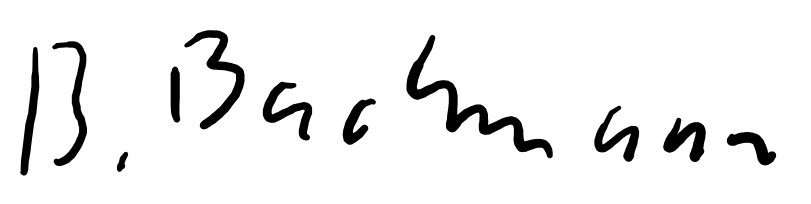
\includegraphics[height=1.5cm,keepaspectratio]{BasilBachmann}\\
	Pascal Baumann & 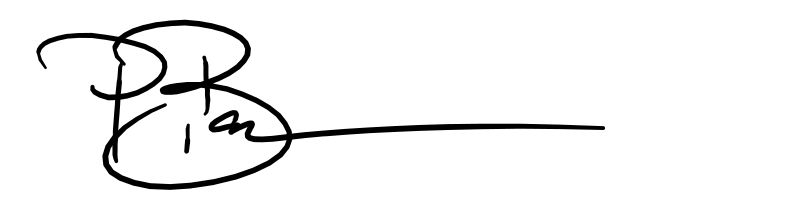
\includegraphics[height=1.5cm,keepaspectratio]{PascalBaumann}\\
	Victor Guntern & 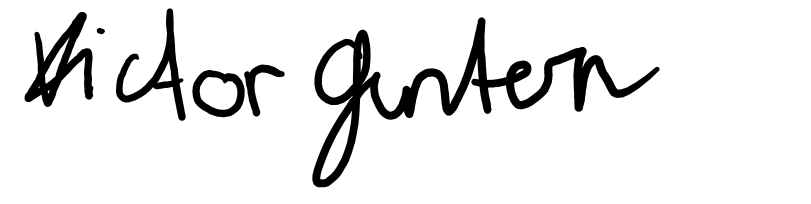
\includegraphics[height=1.5cm,keepaspectratio]{VictorGuntern}\\
	Markus Kempf & 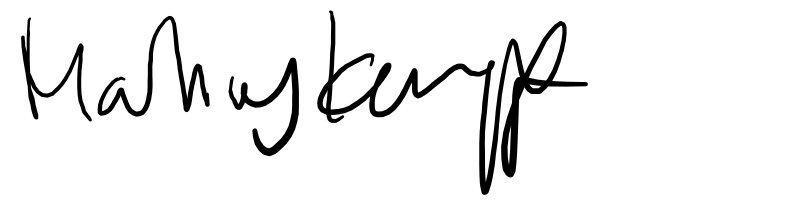
\includegraphics[height=1.5cm,keepaspectratio]{MarkusKempf}\\
	Jan Odermatt & 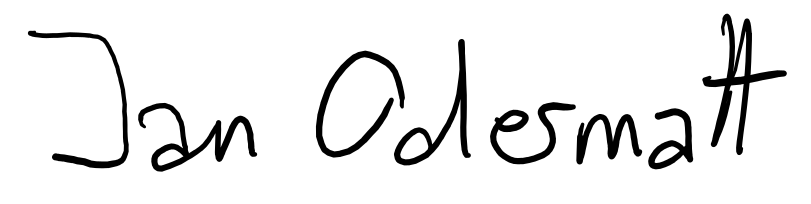
\includegraphics[height=1.5cm,keepaspectratio]{JanOdermatt}\\
	Simon Rohrer &  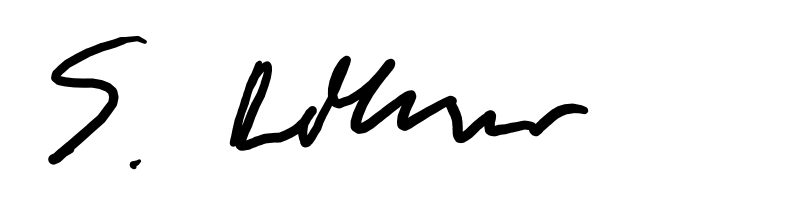
\includegraphics[height=1.5cm,keepaspectratio]{SimonRohrer}\\
\end{tabular}

\newpage

\pagenumbering{roman}
\begin{abstract}
	Im Rahmen des Moduls Produktentwicklung 2 wird ein Funktionsmuster des in PREN01 ausgearbeiteten Konzeptes erstellt. Dabei sind die Fachrichtungen Maschinentechnik, Informatik und Elektrotechnik vertreten. Neben der Realisierung des geplanten Funktionsumfang, steht vor allem auch das gute Abschneiden im Wettbewerb im Vordergrund.
	
	Der Fokus dieses Moduls liegt in dem bauen der Laufkatze und der Funktionalität des ganzen Gerätes. Zudem ist die Projektplanung, die Dokumentation und die Interdisziplinäre Zusammenarbeit sehr wichtig. Das Ziel des Projektes ist es, eine Laufkatze zu entwickeln welche autonom eine Last aufheben und an einer zuvor unbestimmten Position auf eine Zielplatte absetzten kann. Die Position der aufgenommenen Last soll während dem Transport angezeigt werden.
	
	Das Ergebnis dieser Arbeit ist ein Konzept einer Laufkatze, welche mit Seilrollen angetrieben wird. Unterhalb der Aufhängung ist die Montageplatte und die Hubeinrichtung angebracht. Diese besteht aus einem Hacken welcher mit einer geführten Seilwindenkonstruktion gehoben werden kann. Die Zielplatte wird mittels Bilderkennung erkannt und die Distanz mit Ultraschallsensoren und dem Zählen der Schritte von den Motoren.
	
	Am Ende des Moduls wird das geschaffene an einem Wettbewerb von Experten bewertet. Es werden unter anderem die Geschwindigkeit, die Genauigkeit und die fehlerfreie Absolvierung der Aufgaben angeschaut. 
	
\end{abstract}

\chapter*{Versionierung}
\label{ch*:Vers}
\vspace{2em}

\noindent
\begin{tabular}{|c|p{0.7\textwidth}|}
	\hline
	\textbf{Versionsnummer} & \textbf{Beschreibung}\\
	\hline
	0.1 & Erstellung \\
	\hline
\end{tabular}

\tableofcontents

\newpage

\pagenumbering{arabic}

\chapter{Einleitung}
\label{ch:Intro}
Dieses Dokument beschreibt ein Funktionsmuster einer autonomen Laufkatze. Dabei handelt es sich um ein interdisziplinäres Projekt, welches über zwei Semester an der Hochschule Luzern absolviert wurde. In diesem Projekt musste mit einem begrenzten Budget gearbeitet und vielseitige Herausforderungen bewältigt werden.

In der vorhergegangenen Konzeptentwicklung konnte sichergestellt werden, dass alle Anforderungen durch unser Konzept erfüllt werden. Dieses Konzept gilt es nun auszuführen. Zu beginn wurde vor allem auf einen Prototyp hingearbeitet, welcher die Grundfunktionen ausführen konnte. Auf die Details und die autonomen Funktionen wurde erst später eingegangen. 

Wie im vorherigen Modul Produktentwicklung 1 wurde die Dokumentation mit \LaTeX gestaltet, da es sich bewährte.

\section{Kurzbeschrieb Anforderungen}
\label{sec:KurzAnforder}
Das Gerät muss sich autonom entlang eines ansteigenden Drahtseils fortbewegen können. Eine Last muss an einem fix bestimmten Ort aufgehoben werden, ohne Berührung über nachfolgende Hindernisse transportiert und danach möglichst exakt auf einer Zielplatte im Absetzbereich abgesetzt werden (siehe Abb.\ref{fig:Funktionsskizze}).

Nach dem Absetzen der Last muss das Gerät den Zielraum erreichen und den Masten berühren. Die Zielplatte muss das Gerät selbstständig erkennen können. Das Gerät darf nur die Last, das Drahtseil und den zweiten Masten berühren. Nach Aufnahme der Last, muss die aktuelle Position der Last in x-, und z-Richtung in Echtzeit dargestellt werden.

Das Gerät muss innerhalb von zwei Minuten startbereit sein. Die Zeit um den Zielraum zu erreichen liegt bei maximal vier Minuten. Die Abbildung \ref{fig:Ablaufdiagramm} stellt den beschrieben Ablauf anschaulich dar.

In Abbildung \ref{fig:Blockdiagramm} findet sich eine Darstellung der technischen Komponenten und ihren Zusammenhängen.

\chapter{Produktbeschreibung}
% Beschreibung der Komponenten und des Produkts welche wir in PREN02 erarbeiten
\label{ch:Produktbeschreibung}

\section{Beschreibung der Grundfunktion}
\label{sec:GrundBeschrieb}
Die Grundfunktionen des zu bauenden Gerätes sind hauptsächlich das Fortbewegen an einem Drahtseil und das Greifen und Absetzen einer Last. Um die Last zu greifen ist ein Hubmechanismus notwendig, der die Last um mindestens 200mm heben kann. Um die aktuelle Position messen zu können, wird ein Ultraschallsensor verwendet. Die aktuelle Position der aufzuhebenden Last wird auf dem Gerät mit einem Display angezeigt. Eine Kamera wird verwendet, um die vorgegebene Zielplattform zu erkennen. Damit ist das Gerät in der Lage an der richtigen Position über dem Mittelpunkt der Zielplattform zu stoppen. Diese Funktionen laufen bis auf das Startsignal autonom ab.

\begin{figure}[h!]
	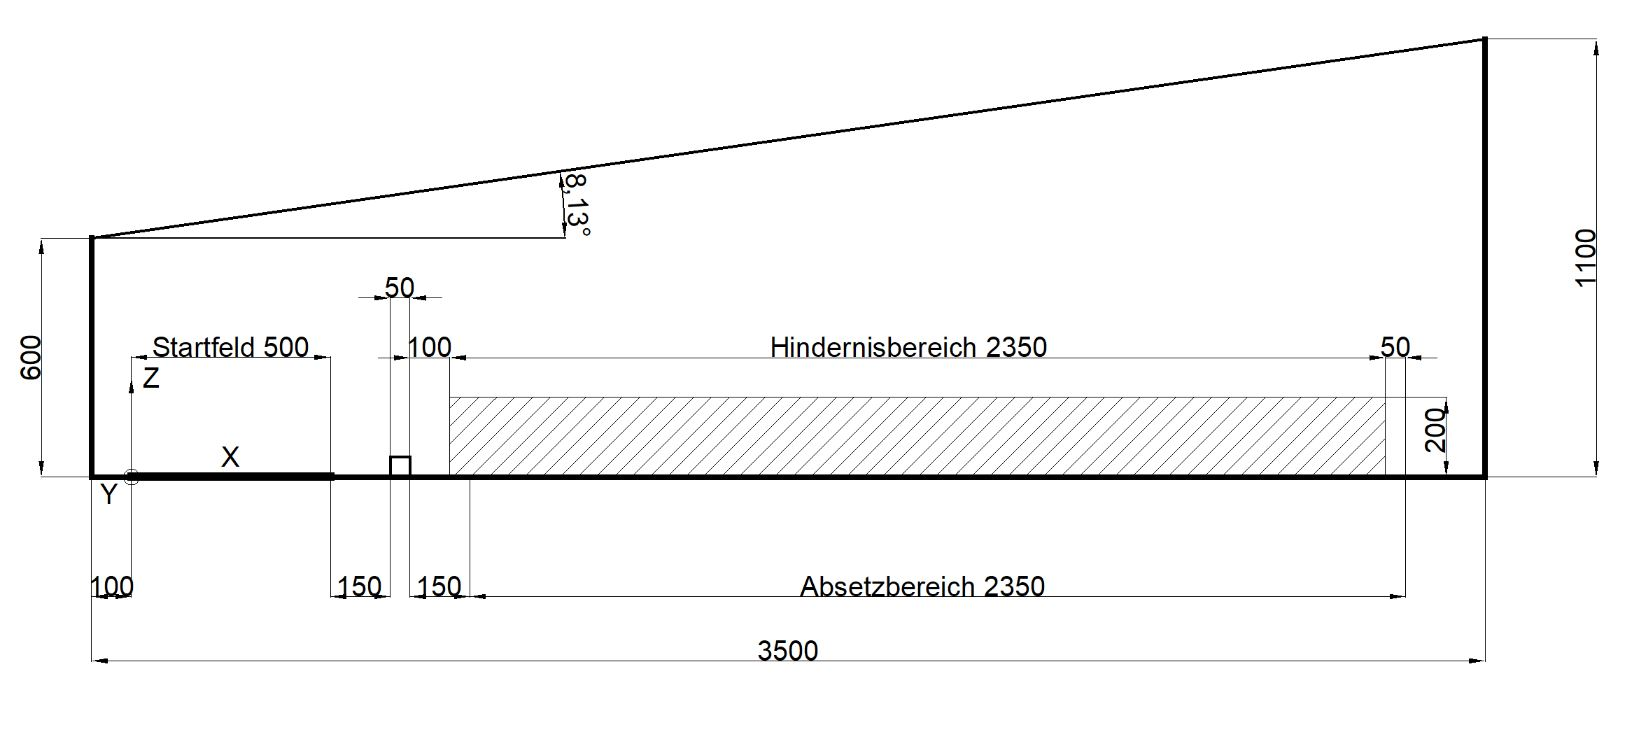
\includegraphics[keepaspectratio,width=\textwidth]{PrenFunktionsskizze}
	\caption{Übersichtsmodell}
	\label{fig:Funktionsskizze}
\end{figure}

\newpage
\section{Ablaufdiagramme}
\label{sec:Ablaufdiagramme}
Der Ablauf der verschiedenen Teilschritte erfolgt gemäss Abbildung \ref{fig:Ablaufdiagramm}.

\begin{figure}[h!]
	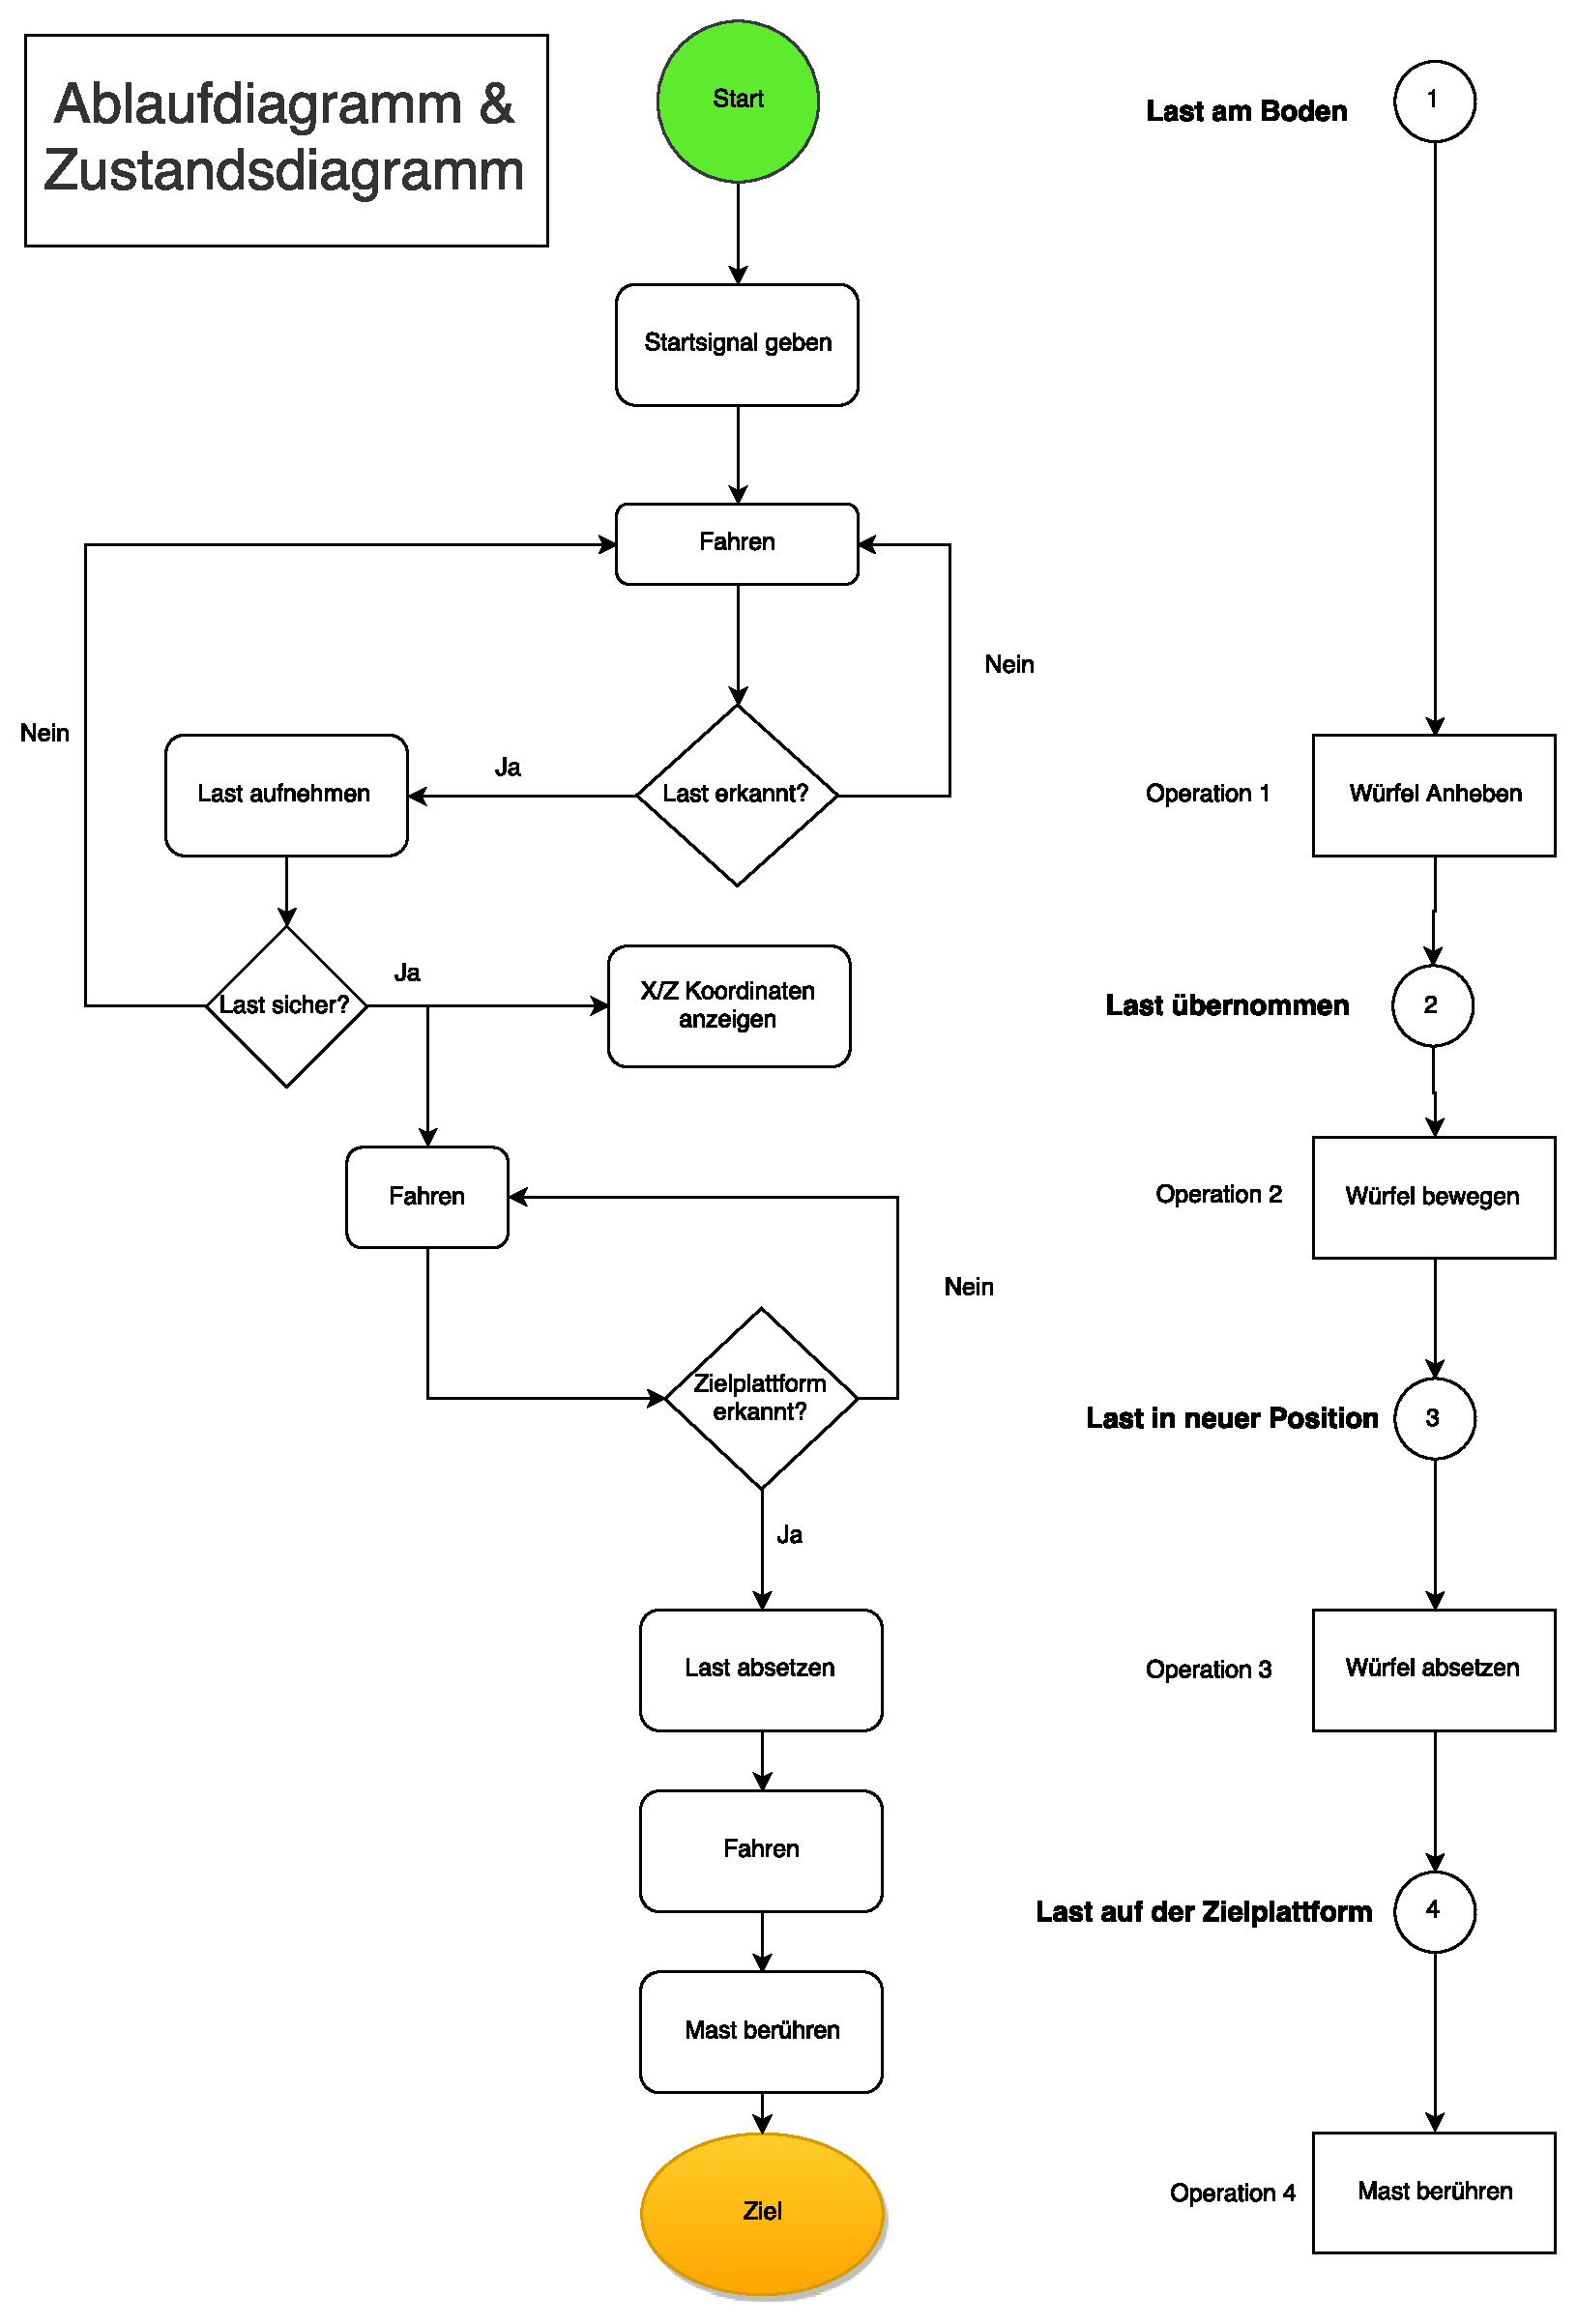
\includegraphics[keepaspectratio,width=\textwidth]{Ablaufdiagramm}
	\caption{Ablauf- und Zustandsdiagramm}
	\label{fig:Ablaufdiagramm}
\end{figure}

\newpage
Im Blockdiagramm (Abb. \ref{fig:Blockdiagramm}) sind die Schnittstellen graphisch dargestellt.

\begin{figure}[h!]
	\centering
	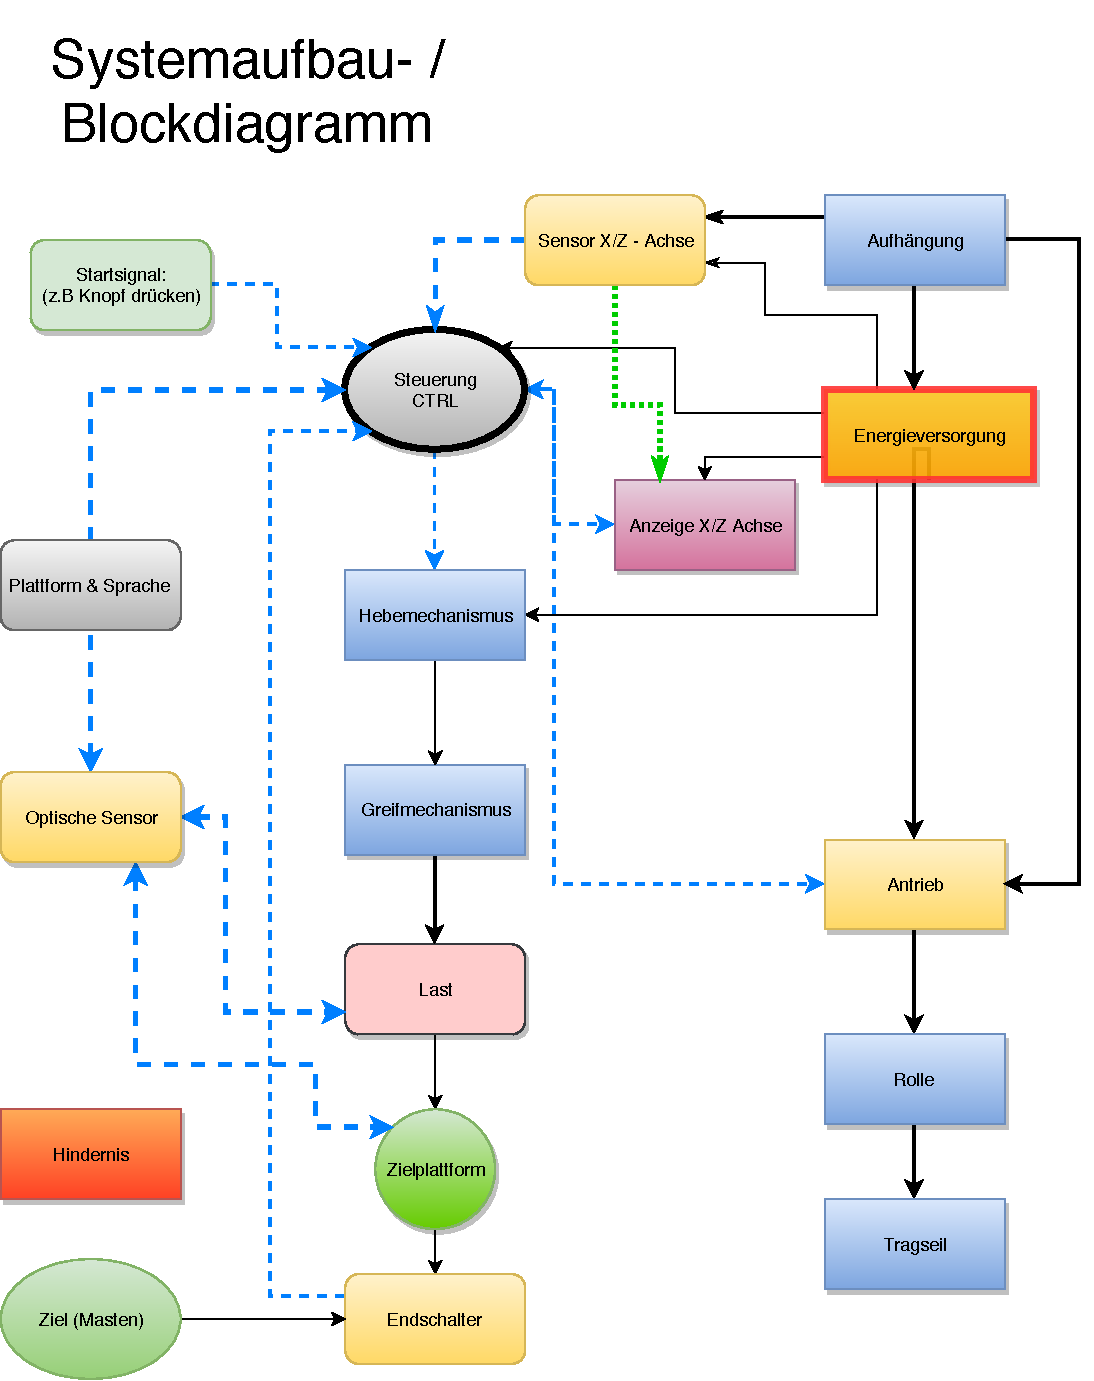
\includegraphics[keepaspectratio,width=\textwidth]{Blockdiagramm}
	\caption{Blockdiagramm}
	\label{fig:Blockdiagramm}
\end{figure}

\section{Komponenten}
\label{sec:Pren02Komponenten}

\begin{figure}[h!]
	\centering
	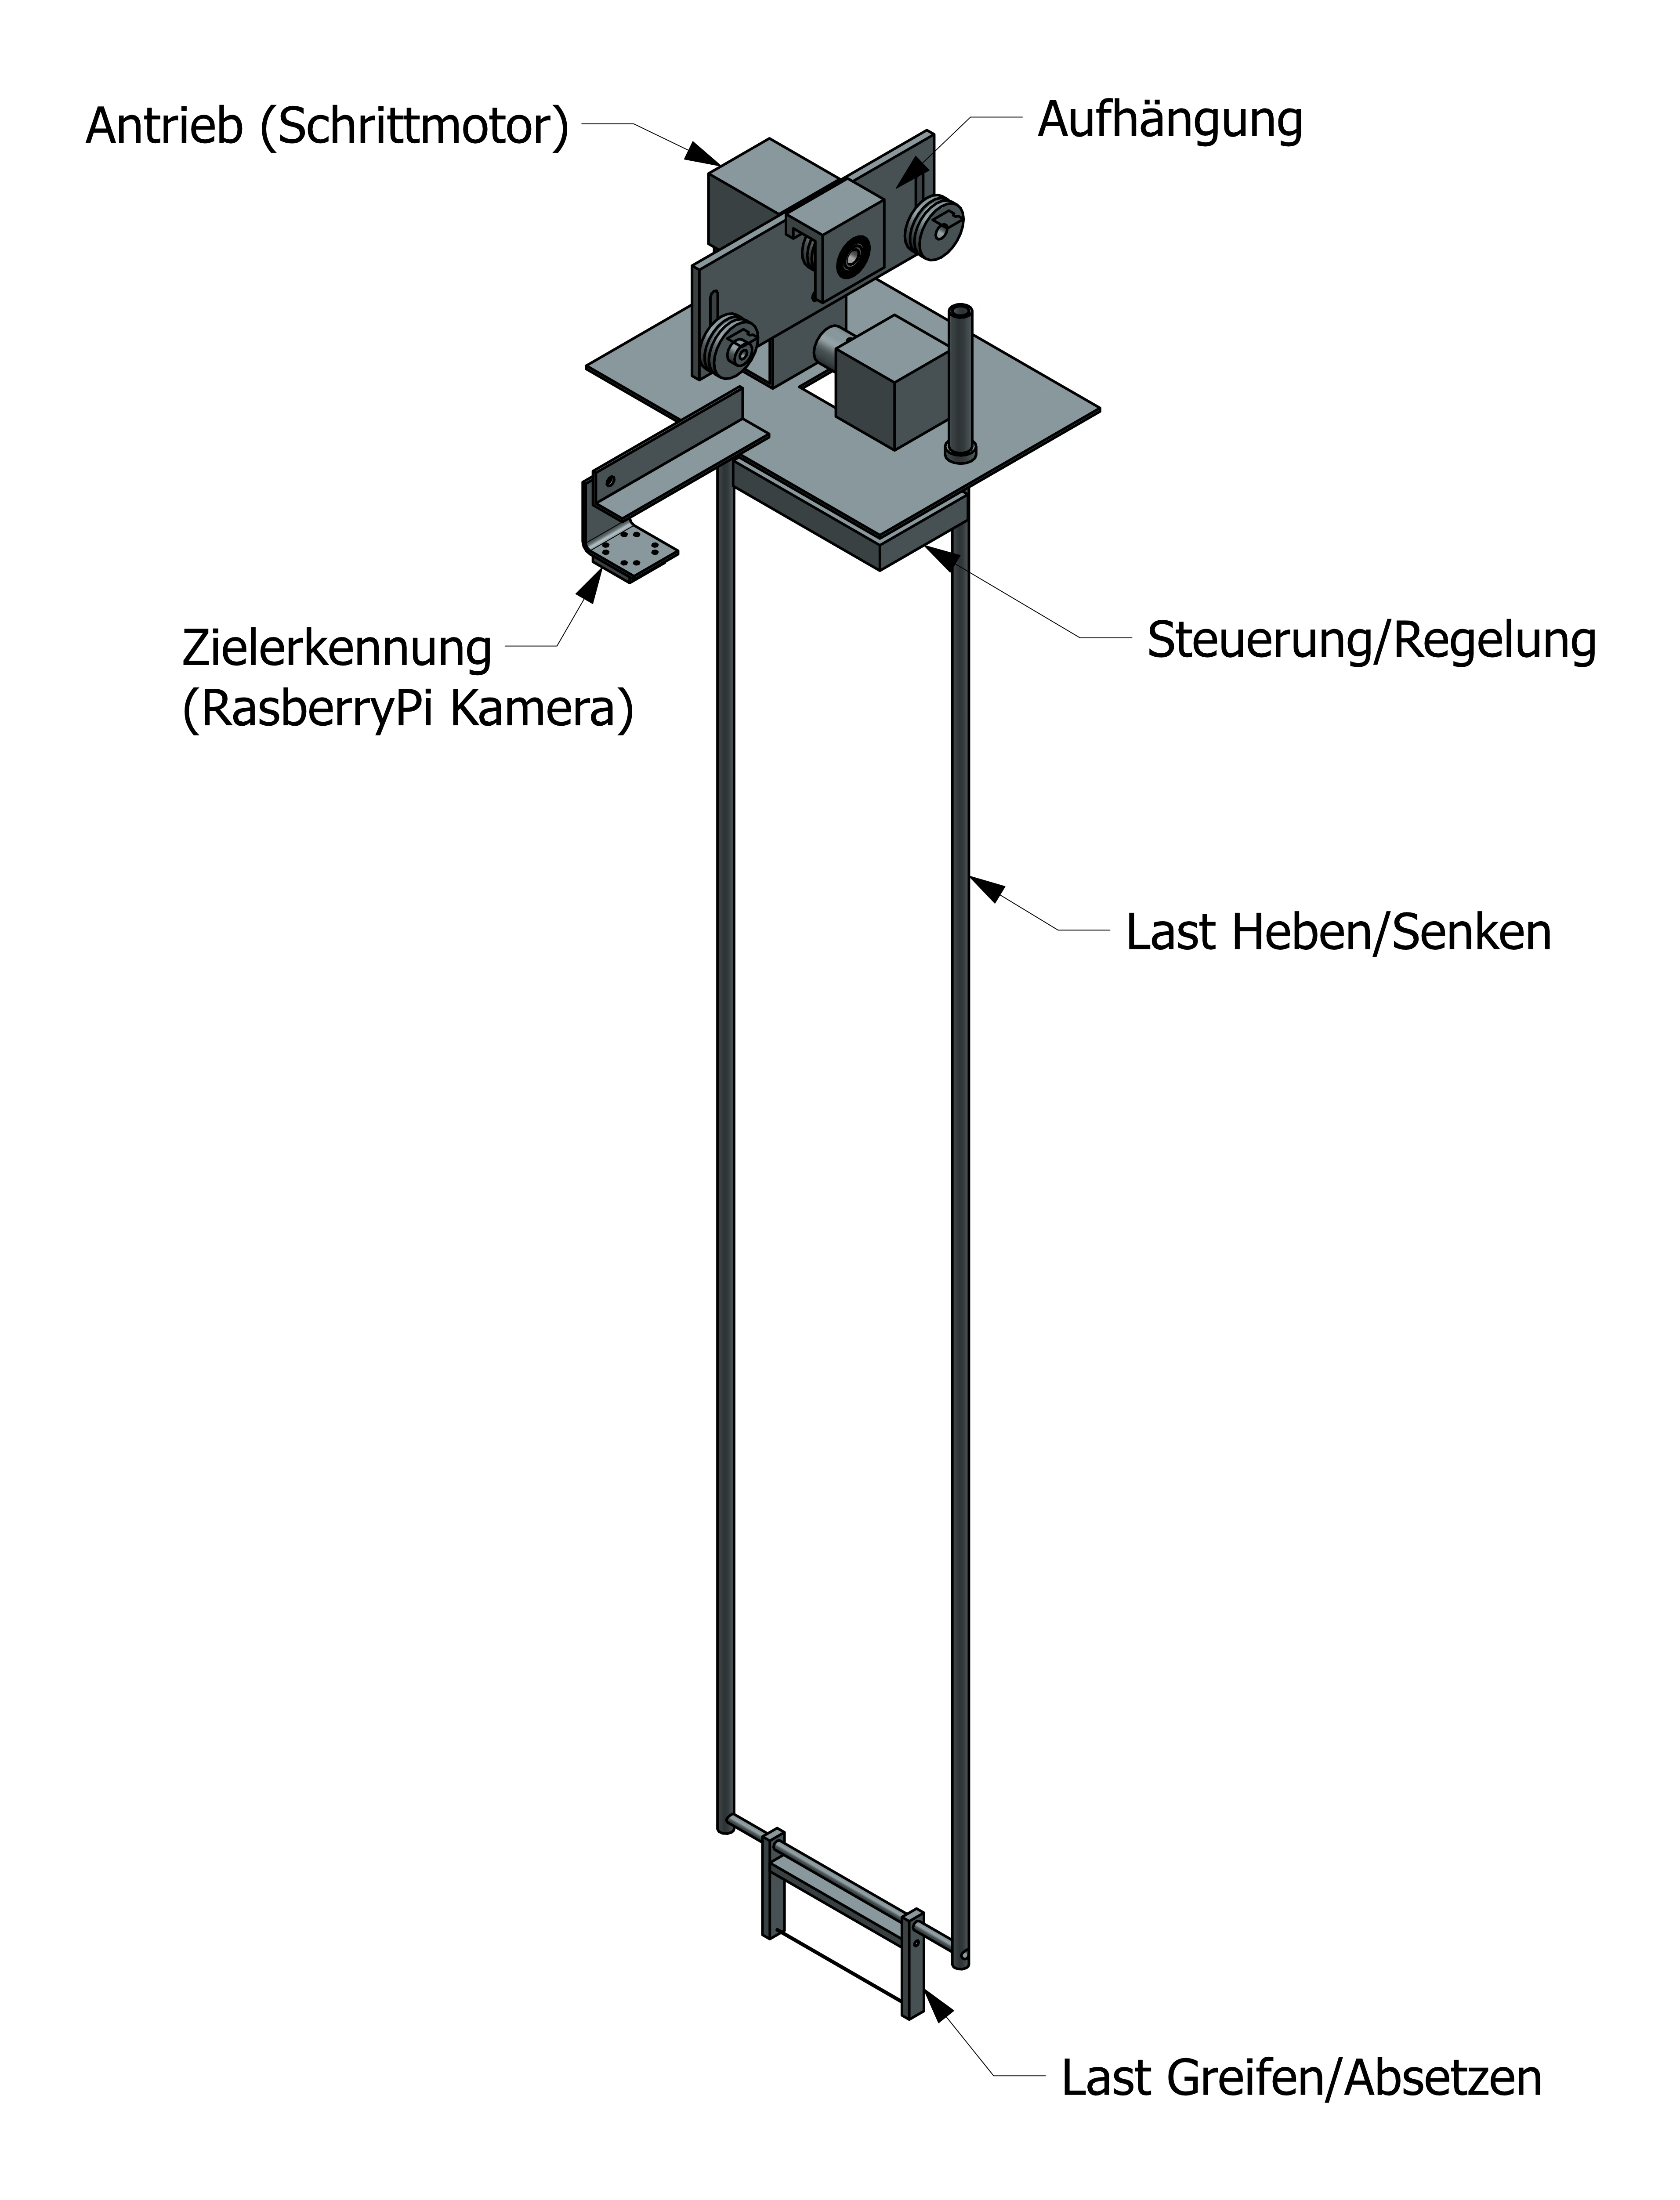
\includegraphics[height=0.5\textheight,keepaspectratio]{marku_103000_bg-00_ze1}
	\caption{Skizze unseres Lösungskonzeptes}
	\label{fig:LoesungsKonzept}
\end{figure}

\newpage

\subsection{Aufhängung}
Durch die unten gelenkige und gedämpft gelagerte Aufhängung kann die Winkeländerung, welche durch den Seildurchhang verursacht wird, kompensiert werden. Dabei hängt die Last durch den Schwerpunkt immer senkrecht nach unten. Durch das Gelenk (ähnlich wie bei einer Gondelbahn) wird der ganze Aufbau aber empfindlich gegen pendeln, weil das Gelenk kein Drehmoment aufnehmen kann. Dieses wird beispielsweise durch die Beschleunigung bei Anfahren oder Abbremsen erzeugt. Das Gelenk wird durch zwei Löcher und eine Schraube mit einer Sicherungsmutter realisiert. Zudem kann sich, je nach Aufbau, der Schwerpunkt der Laufkatze beim Anheben und Absetzen der Last ändern, was wiederum ein Drehmoment erzeugt. Mit Dämpfern kann das Drehmoment aufgenommen und ein Pendeln minimiert werden. Diese Dämpfer werden dann, im Prinzip einer Pendelstütze in der Mechanik, am einen Ende am Antrieb und am anderen Ende an der Aufhängung montiert. Zudem soll der Dämpfer möglichst horizontal angestellt sein, damit er die Pendelbewegung aufnehmen kann. In der Aufhängung werden der Hubmotor, die elektrischen Komponenten, die Energieversorgung und die Führungen der Hubeinrichtung angebracht. Diese besteht aus zwei Linearführungen, durch welche zwei Stäbe in einem Rohr hoch und hinuntergefahren werden. Weiter werden, je nach Notwendigkeit, Ausgleichsgewichte auf der Aufhängung positioniert, damit die Laufkatze zentral unter dem Seil hängt. Die Aufhängung wird komplett aus Aluminium gefertigt.

\subsection{Antrieb}
Der Antrieb auf dem Seil wird mit drei Rädern aus Aluminium ausgeführt. Das mittlere Rad ist das angetriebene Rad. Es wird direkt von einem Schrittmotor angetrieben. Dies setzt voraus, dass die Achse des Motors um den Radius des Antriebsrades über dem Seil sein muss. Dies hält die Ausfallwahrscheinlichkeit tief, da keine Riemen-, oder Zahnradübersetzung notwendig sind. Zudem kann auch der Schlupf klein gehalten werden. Weil der Motor aber über dem Seil liegt, ist auch der Schwerpunkt des gesamten Gerätes höher. Dies macht den Lastausgleich schwieriger und begünstigt Schwingungen.
\\
Vor und hinter dem Antriebsrad sind im Abstand von 7cm zwei Führungsräder angebracht. Diese sind in der Höhe verstellbar und müssen manuell im voraus eingestellt werden. Die Aufgabe dieser Räder ist die Schwingung in x-Richtung zu minimieren und den Druck des Seiles auf das Antriebsrad zu erhöhen. Letzteres hat zur Folge, dass die Reibkraft sich erhöht und somit der Schlupf und die Gefahr von Rutschen auf dem Seil minimiert wird. Um die Reibkraft zusätzlich zu erhöhen, wird die Laufrille des Antriebsrades aus Aluminium mit einer Gummibeschichtung versehen.

\subsection{Kamerahalterung} %todo Abmasse halterung anpassen
Die Kamera ist etwa 20 Zentimeter vor der Seilwinde für den Hub angebracht. Dafür wurde ein 11 Zentimeter langes Winkelprofil aus Aluminium an der Grundplatte angeschraubt. An diesem ist ein kleiner Aluminiumwinkel befestigt, der die Kamera hält. Dieser ist schwenkbar, damit die Kamera optimal ausgerichtet werden kann. Dabei ist essentiell wichtig, dass die Grundplatte immer Parallel zum Boden liegt, da sonst die Kamera falsche Daten liefern würde und somit die Genauigkeit beim Absetzen stark beeinträchtigen würde. Die RasPi-Kamera wird mit 4 Schrauben an dem Winkel befestigt. Zusätzlich zu der Kamera werden auch die beiden Ultraschallsensoren und der Endschalter an der Halterung befestigt.

\subsection{Regelung und Steuerung}
Als Kern der elektronischen Steuerung wird das \textit{LoFive} Board verwendet, welches mit dem \textit{SiFive Freedom E310} Mikroprozessor bestückt ist. Dieser wurde nach dem offenen Standard der RISC-V Foundation konstruiert und ist daher für jeden einsehbar. Als Programmiersprache wird voraussichtlich Rust verwendet.

Über das Board werden zwei Schrittmotoren-Treiber sowie ein LCD-Display angesteuert. Zur Rückmeldung werden zwei Ultraschallsensoren und ein \textit{Raspberry Pi 3 Model B} (RasPi) verwendet.

Weil die Steuerung vom RasPi die Richtung und Distanz zur Zielplattform übermittelt, kann das System als Regelungssystem betrachtet werden. Solange das Ziel nicht erkannt wird, soll das Gerät mit maximaler Geschwindigkeit fahren. Mit der Erkennung des Ziels wird das Gerät immer langsamer und stoppt über dem Zielfeld. Mit diesem System wird ein effektives Anfahren des Ziels erreicht. Zum Starten und Stoppen des Geräts wird ein Schalter und ein Taster verwendet.

\subsection{Positionsanzeige}

Auf dem LCD-Display werden die Koordinaten in x- sowie z-Richtung dargestellt. Die x-Koordinate wird mithilfe des Schrittmotors und zusätzlich mit einem Ultraschall-Distanzsensor bestimmt. Die z-Koordinate wird mittels einem weiteren Ultraschall-Sensor erkannt. Bei z-Koordinate muss jedoch noch einen Betrag abgezogen werden, da der Ultraschallsensor an der Grundplatte befestigt ist und die angezeigten Koordinaten müssen die der transportierten Last sein. Wieviel abgezogen werden muss, wird über den Hubschrittmotor berechnet. Sobald die Daten des Ultraschall-Sensors stark von der Durchhangsberechnung abweicht, sollen die Daten der Durchhangsberechnung angezeigt werden. Damit können Fehler verhindert werden, welche durch Hindernisse auftreten.

\newpage
\subsection{Zielerkennung}
\subsubsection{Systemübersicht}

\begin{figure}[h!]
	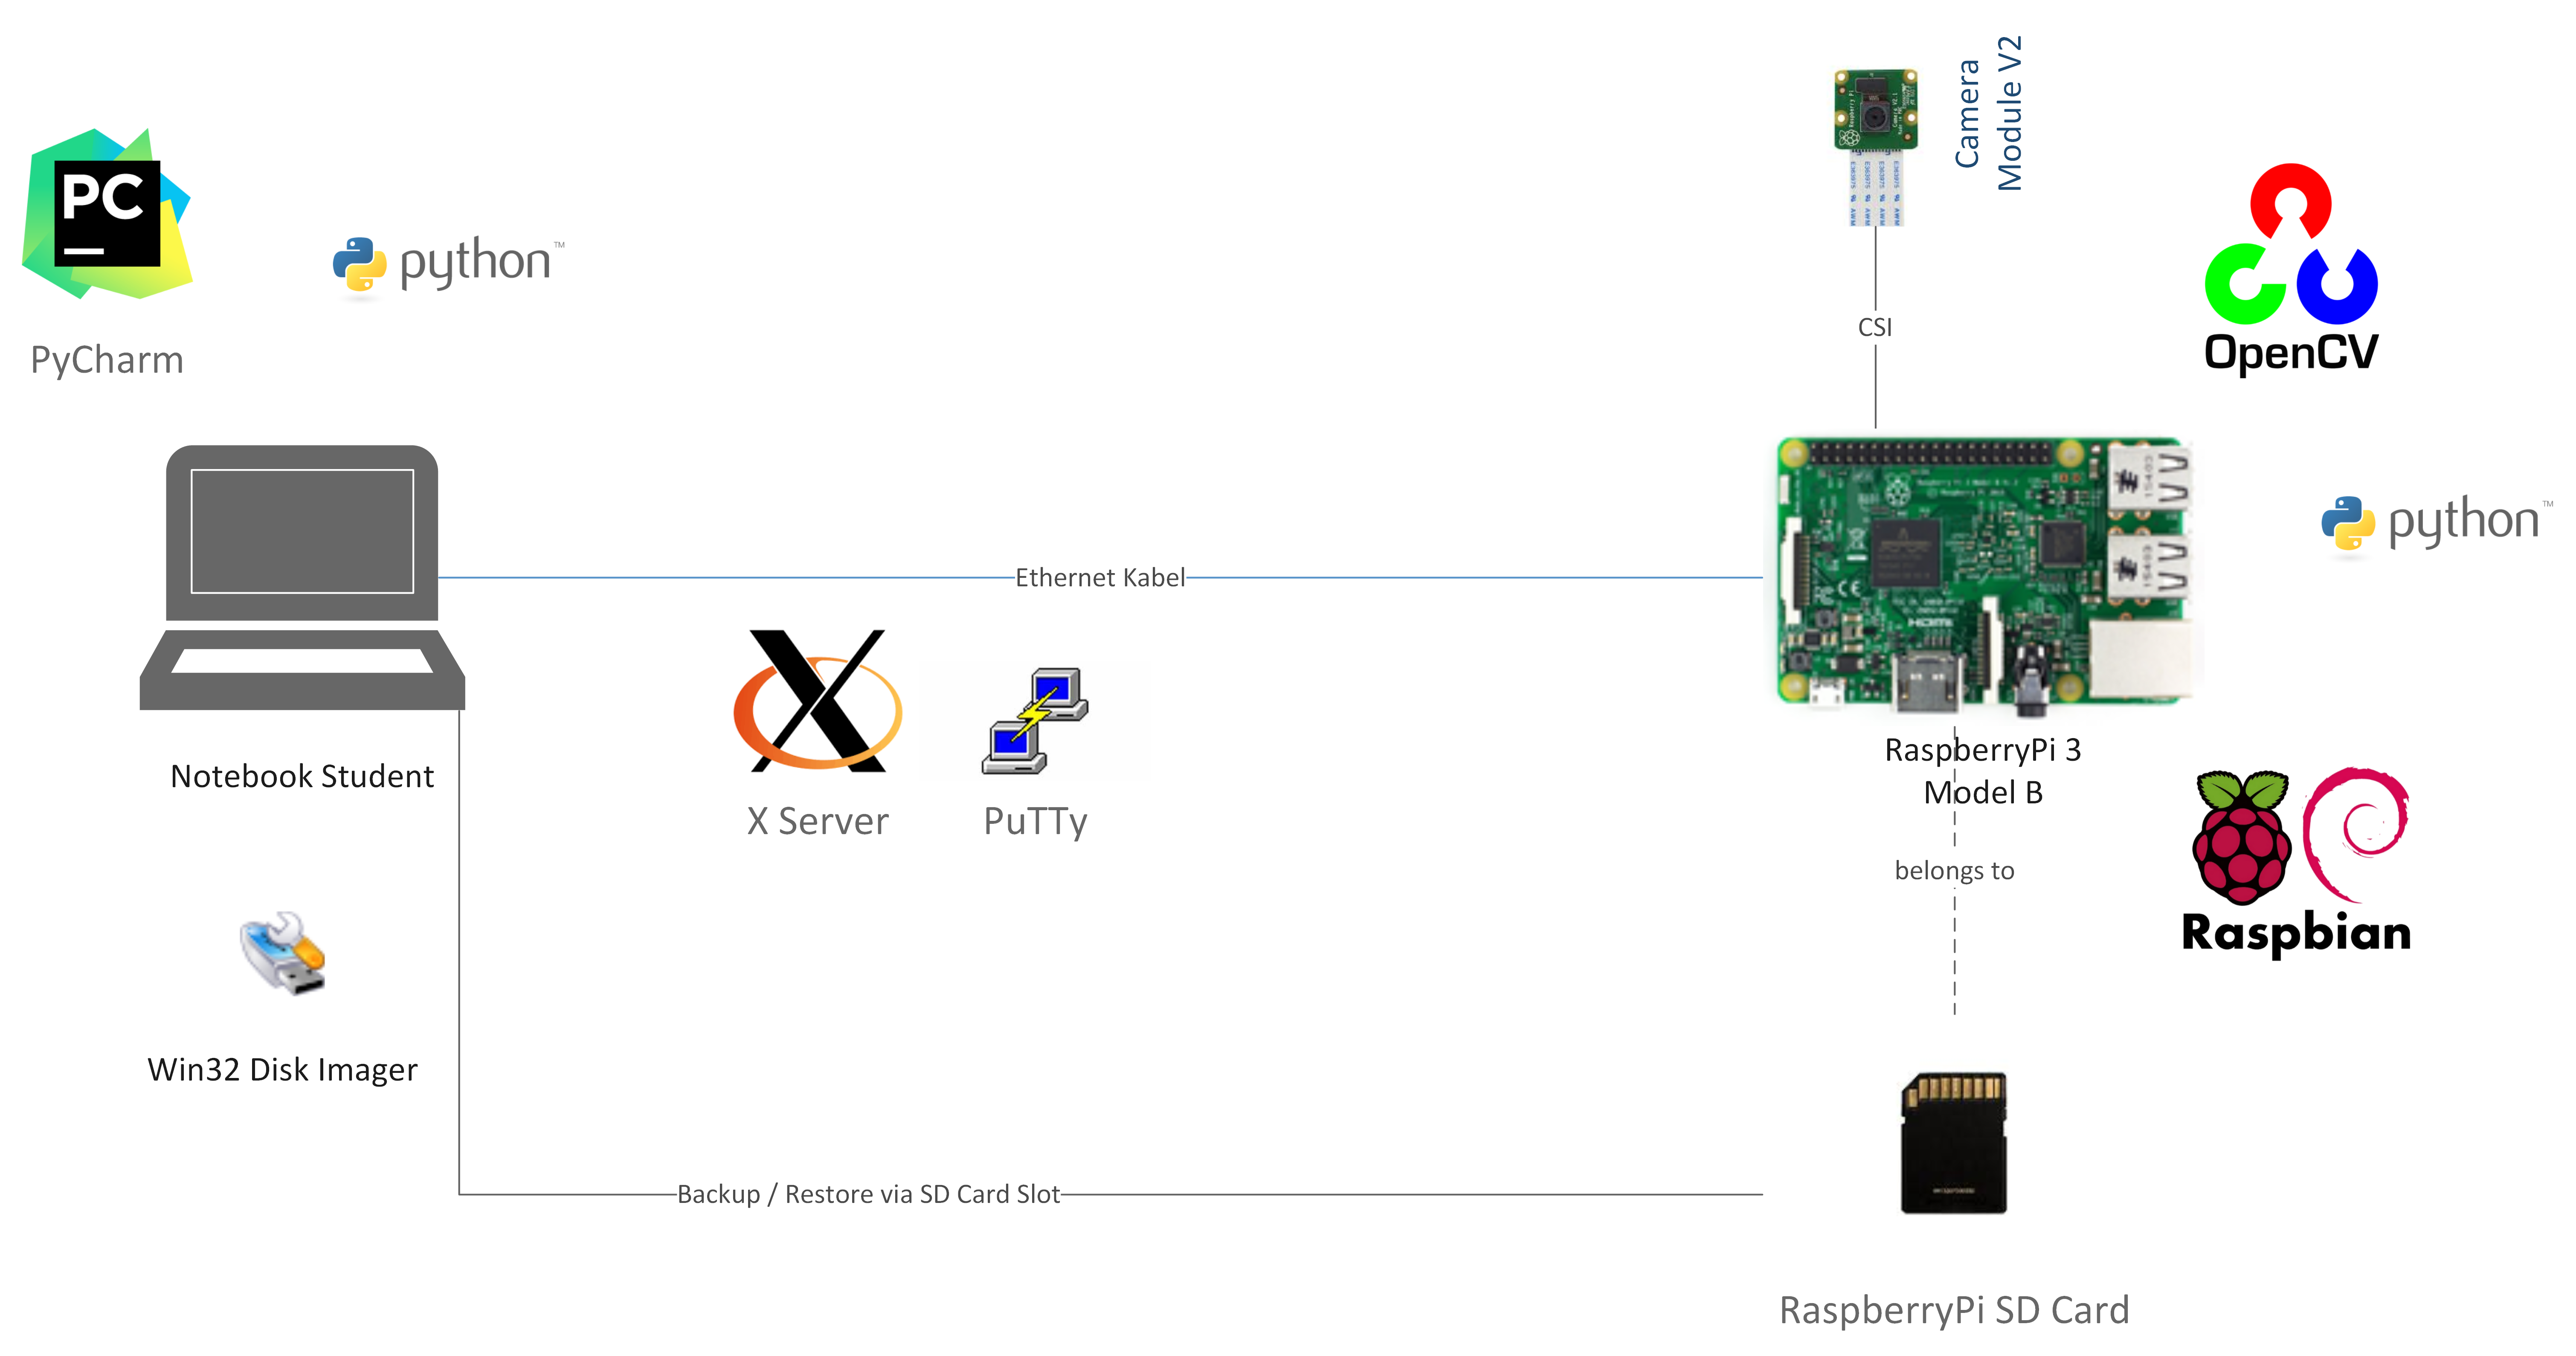
\includegraphics[keepaspectratio,width=\textwidth]{TargetRecOS}
	\caption{Systemübersicht}
	\label{fig:Systemuebersicht}
\end{figure}

Auf dem Raspberry Pi wird als Grundinstallation das Betriebssystem Raspian installiert. Darauffolgend werden Module für Python (Version 2) und OpenCV (Version 3) für die Bilderkennung hinzugefügt.
Um auf das Raspberry Pi zugreifen zu können, wird einerseits PuTTy benutzt um eine SSH Verbindung aufzubauen, andererseits benötigen wir den X Server für das Streaming des Kamerabildes.
Um den aktuellen Stand (das Abbild, Image) des RaspberryPi zu speichern und gegebenenfalls wiederherstellen zu können, wird die SD Karte in ein Studentennotebook gelegt und mithilfe Win32 Disk Imager kopiert.

Auf dem jeweiligen Notebook wird PyCharm als IDE benutzt und als Programmiersprache Python verwendet.

Das System muss den Ablauf in Abbildung \ref{fig:AblaufZielerkennung} umsetzen können.

\begin{figure}[h!]
	\centering
	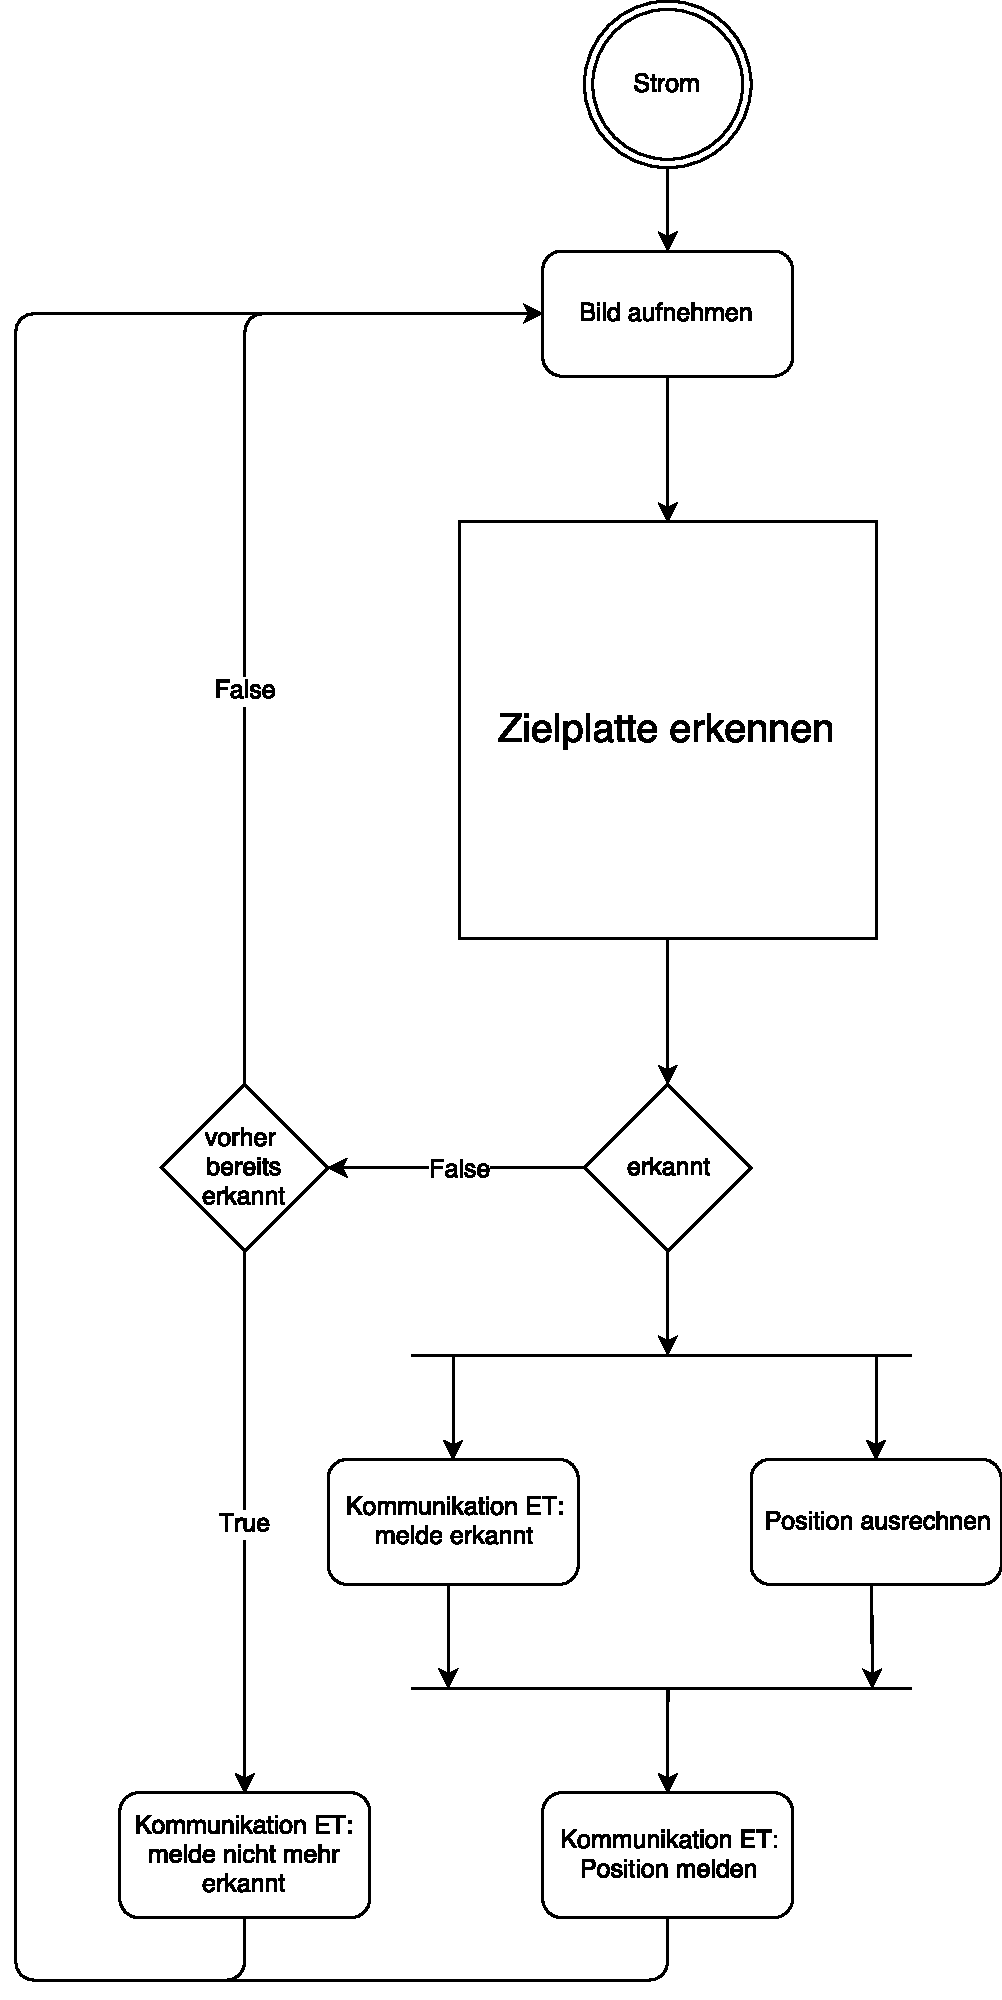
\includegraphics[keepaspectratio,height=0.8\textheight]{Ablaufdiagramm_ModusOperandi}
	\caption{Ablaufdiagramm Zielerkennung}
	\label{fig:AblaufZielerkennung}
\end{figure}

Der Schritt \textquotedblleft Zielplatte erkennen\textquotedblright\ wird im Kapitel \ref{ssec:bilderkennung} ausführlich beschrieben.

Jene Schritte mit der Bezeichnung \textquotedblleft Kommunikation ET\textquotedblright\ werden im Kapitel \ref{ssec:kommunikation} detailliert beschrieben.

\subsubsection{Bilderkennung}
\label{ssec:bilderkennung}

\begin{figure}[h!]
	\centering
	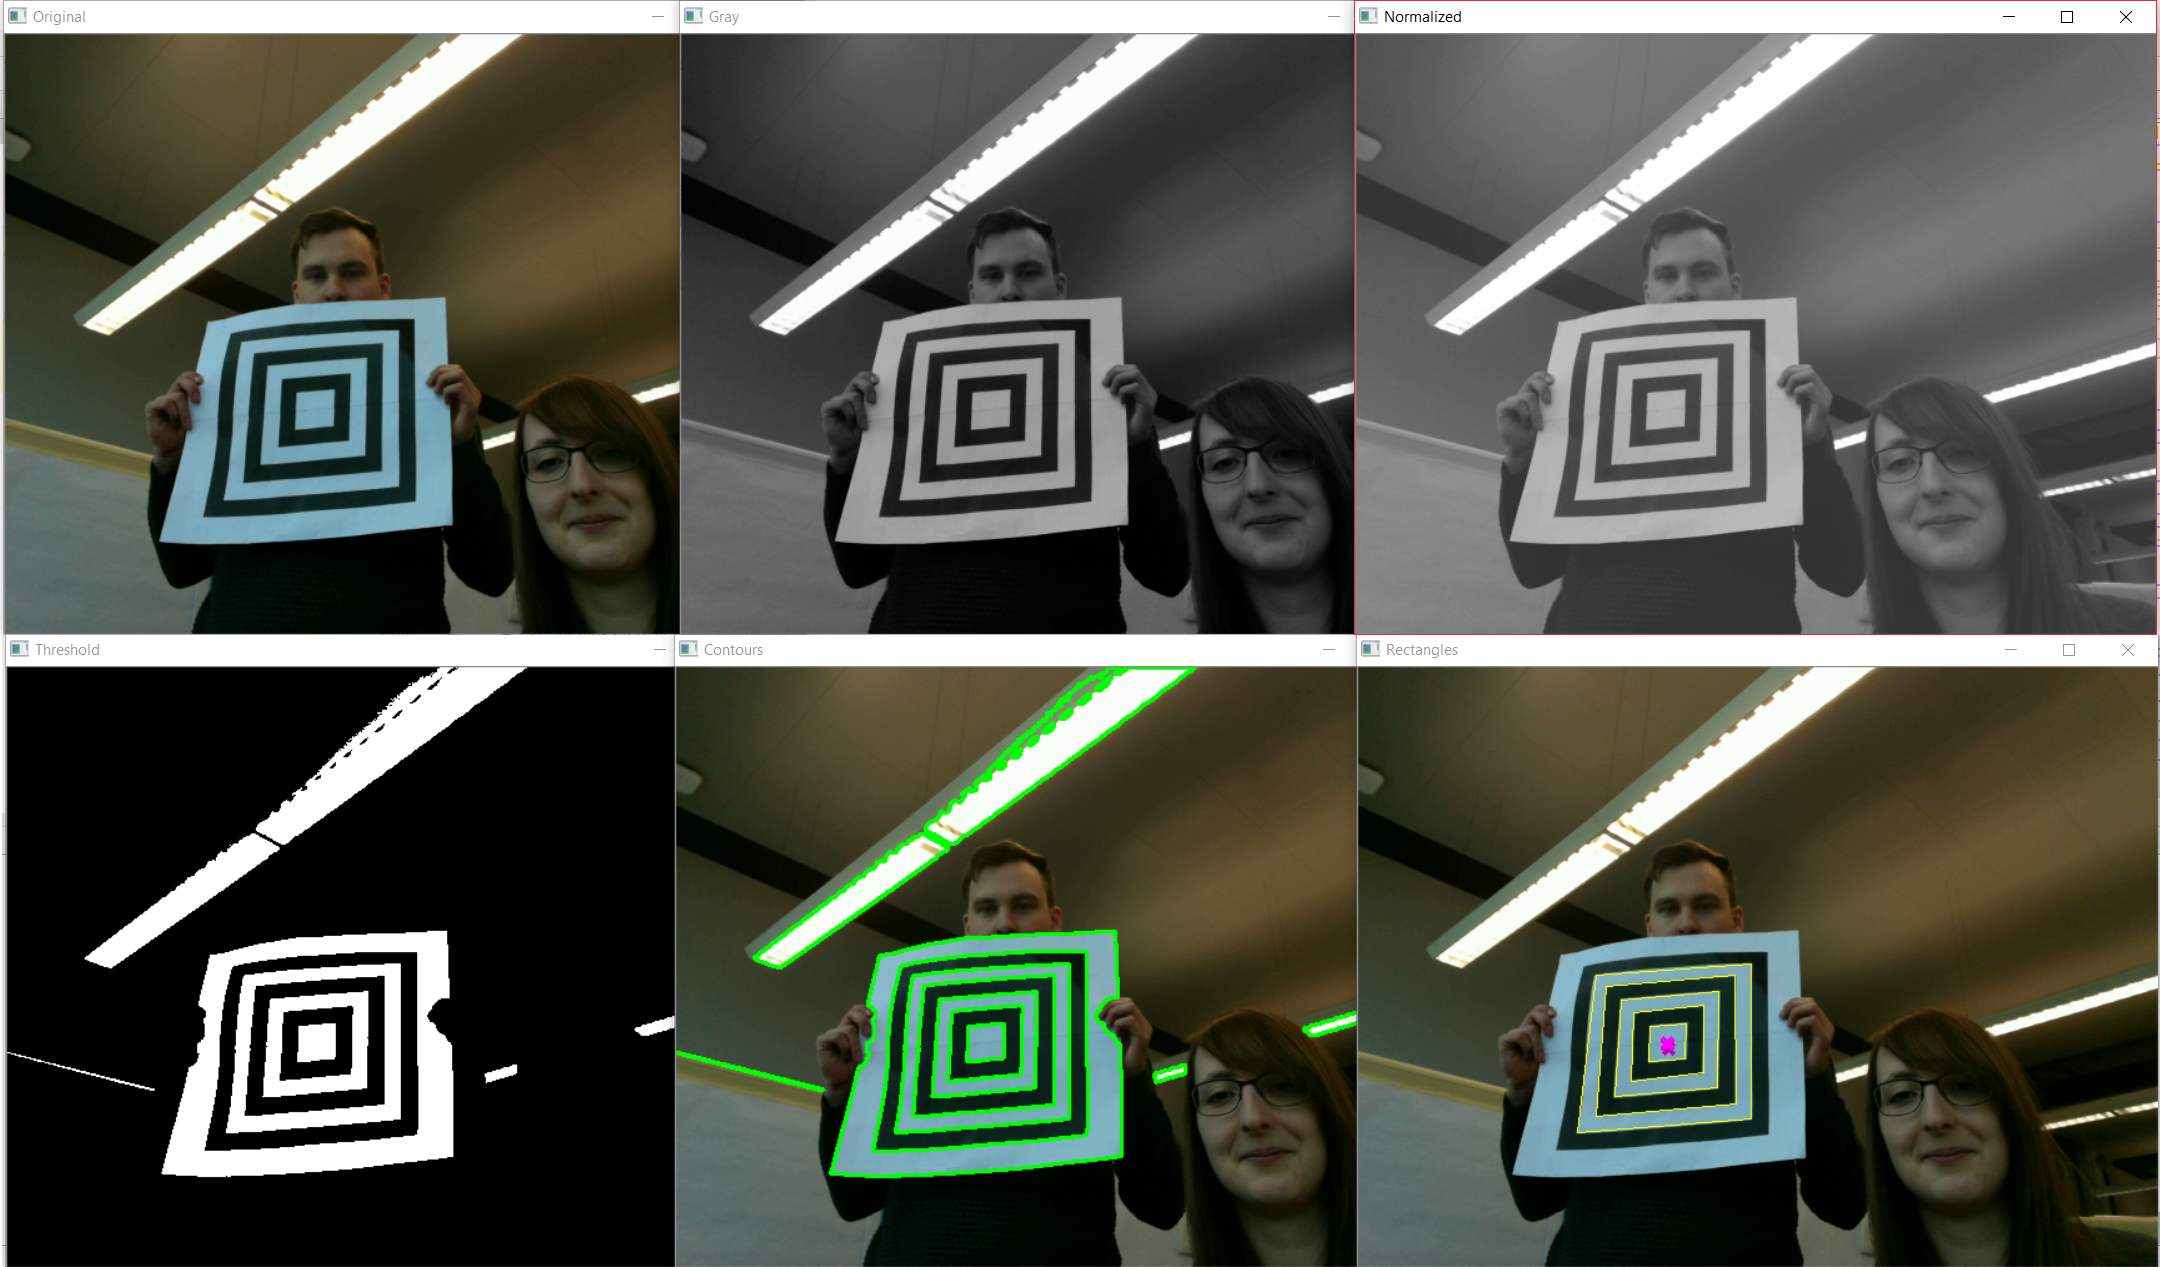
\includegraphics[keepaspectratio,width=\textwidth]{BilderkennungAblauf}
	\caption{Aufnahmen der einzelnen Schritte der Zielerkennung}
	\label{fig:AufnahmeZielerkennung}
\end{figure}

Die Erkennung (in Abbildung \ref{fig:AufnahmeZielerkennung} dargestellt) läuft wie folgt ab:

\begin{itemize}[noitemsep]
	\item[-] Videoframe aufnehmen
	\item[-] Frame in Graustufen umwandeln
	\item[-] Helligkeit durch CLAHE\footnotemark normalisieren
	\item[-] Binären Schwellenwertfilter anwenden
	\item[-] Konturen ausfindig machen
	\item[-] Polygone ausfindig machen
	\item[-] Nur Rechtecke weiter beachten
	\item[-] bestimmte Anzahl Rechtecke mit dem gleichen Mittelpunkt ausfindig machen
	\item[-] Zielplatte erkannt
\end{itemize}

\footnotetext{contrast limited adaptive histogram equalization}

Dieser Ablauf wird in Abbildung \ref{fig:ZielerkennungAblauf} noch genauer dargestellt.

\begin{figure}[h!]
	\centering
	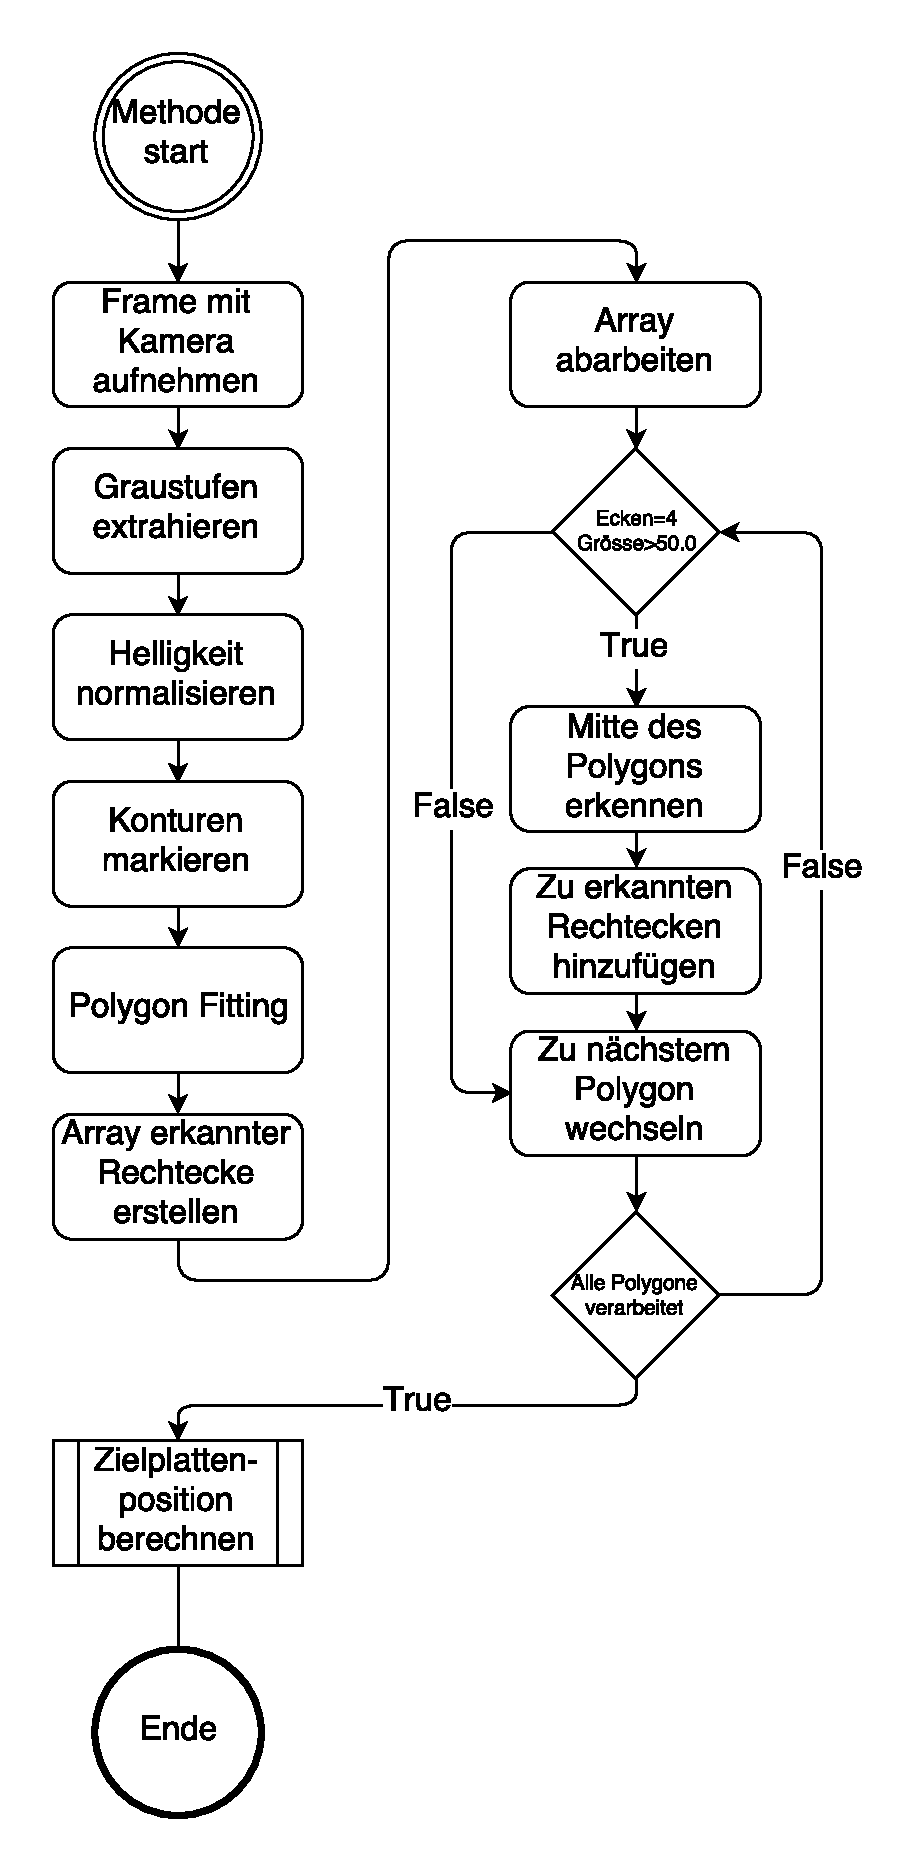
\includegraphics[keepaspectratio,height=0.6\textheight]{ZielplatteErkennen}
	\caption{Ablaufdiagramm Zielerkennung}
	\label{fig:ZielerkennungAblauf}
\end{figure}

\newpage

\subsubsection{Kommunikation zwischen Boards}
\label{ssec:kommunikation}
Zwischen dem Raspberry Pi und dem Elektronikerboard soll der Informationsaustausch über eine serielle Schnittstelle erfolgen.

Für die Verwendung einer Kommunikation mit einer asynchronen, seriellen UART-Schnittstelle können jeweilige PINs verwendet werden.

Wie in Abb. \ref{fig:RaspberryPins} dargestellt sind dies Pin 8 (Tx) und Pin 10 (Rx).
\begin{figure}[h!]
	\centering
	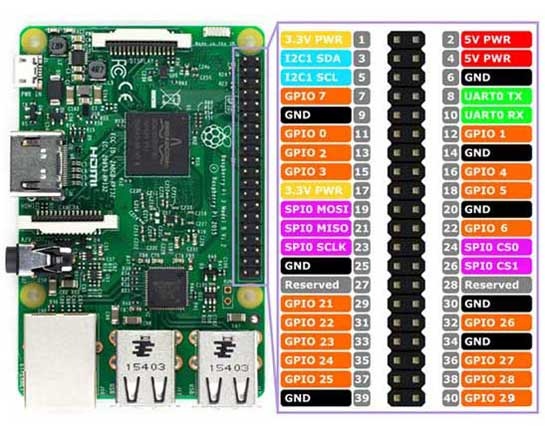
\includegraphics[keepaspectratio, width=0.7\textwidth]{raspberry_pi3_model_b_pin_diagram.jpg}
	\caption{RaspberryPi Pin Diagram}
	\label{fig:RaspberryPins}
\end{figure}

Die Pins können für Testzwecke direkt via Kabel miteinander verbunden werden. Im Endausbau soll diese Verbindung jedoch über einen eigens angefertigten Print laufen. So wird auch sichergestellt, dass beide Boards eine gemeinsame Erdung besitzen.

UART muss auf dem Raspberry Pi manuell aktiviert werden.  Zusätzlich muss das integrierte Bluetooth-Modul deaktiviert werden, sodass die genannten Ports nicht \textquotedblleft miniUART\textquotedblright\ verwenden.

Für die serielle Übertragung müssen Baudrate, Port, Databits, Parity Check, Stopbits und flow control sowie ein genaues Nachrichtenformat definiert werden. Die Programmierung dieser wird auf dem RaspberryPi mit Hilfe des Python Moduls \textquotedblleft pySerial\textquotedblright\ realisiert.

\newpage

\subsection{Last greifen und absetzen}

Das Greifen der Last erfolgt über einen gelenkig gelagerten Haken. Die gelenkige Lagerung ermöglicht einen grösseren Toleranzbereich in Richtung Z-Achse zum Anheben der Last. Versuche haben gezeigt, dass bei Berührung der Last der Greifer nach hinten gekippt wird und durch das Vorwärts bewegen des Fahrzeuges sich in den Haken der Last einfädelt. Siehe \textquotedblleft Testprotokoll Last greifen mit Haken\textquotedblright und \textquotedblleft Testprotokoll Last absetzen mit Haken\textquotedblright  im Anhang \ref{app:ch:Versuche}. Durch einen gekrümmten Draht an der Unterseite des Greifers wird sicher gestellt, dass die Last nach dem Anheben mittig zentriert und durch die Fahrt nicht verschoben wird.

Nachdem das Fahrzeug die Zielplattform erreicht hat, wird die Last vorsichtig abgesetzt. Das Ausfädeln des Drahtes aus dem Haken erfolgt durch eine Rückwärts\-bewegung des Fahrzeuges.

Der Greifer wird aus Aluminium gefertigt. Dieser besteht aus gebogenem Flachmaterial, durch welchen im oberen Bereich eine Drehachse und im unteren Bereich ein gebogener Draht durch ein Loch geführt wird. Die Drehachse dient zudem noch als Befestigung des Greifers an die Hubvorrichtung.

\subsection{Last anheben und senken}
Die Last wird mithilfe einer Seilwinde angehoben, welche mit einem Schrittmotor angetrieben wird. Dieser ist auf der Befestigungsplatte positioniert. Auf der Motorachse ist eine Seiltrommel aus Aluminium befestigt, welche einen Nylonfaden aufwickelt. Das Ende des Fadens ist direkt am Greifer befestigt. Da ein loses Seil stark in Schwingung geraten kann, wird zusätzlich eine Führung mit zwei Stäben aus Kohlenstofffasern verwendet. Auf der Befestigungsplatte sind dafür Führungsrohre montiert. Um den Widerstand zwischen der Führung und dem Stab so klein wie möglich zu halten, wird das Führungsrohr geschmiert. Damit sichergestellt werden kann, dass sich die Stäbe synchron bewegen, wird eine Querverstrebung eingebaut. Damit kann ein Verkanten der Stäbe aufgrund von ungleicher Hubgeschwindigkeit der Stäbe ausgeschlossen werden. Mit diesen Massnahmen können die Schwingungen stark minimiert und eine Verdrehung des Greifers verhindert werden. Dank diesem Aufbau kann der Greifer genauer geführt werden und somit der Transport der Last optimiert ablaufen.

\subsection{Ultraschallsensor}
%todo Beschreibung Ultraschallsensor
Für die Distanzmessung werden in x-Richtung und y-Richtung je ein Ultraschallsensor verwendet. Die Ultraschallsensoren des Typs HC-SR04 weisen eine Messdistanz zwischen zwei Zentimeter und bis zu fünf Meter auf. Die Genauigkeit wird mit drei Millimetern Abweichung angegeben. Dies ist ausreichend für die geplante Anwendung. Ausgelesen und verarbeitet werden die Informationen auf dem Arduino.

\subsection{Schrittmotoren}
%todo Beschreibung Schrittmotoren

\subsection{RasPi-Kamera}
%todo Beschreibung Kamera

\subsection{Arduino}
%todo Beschreibung Arduino DUE

Als Unterstützung zum RasPi wird ein Arduino Due eingesetzt. In Vergleich zum kleineren Arduino Uno liegt der Vorteil in der grösseren Anzahl Ein und Ausgänge, womit es sich vor allem für grössere Projekte anbietet.



\begin{itemize}[noitemsep]
	\item Atmel SAM3X8E ARM Cortex-M3 CPU (32-bit ARM controller)
	\item 512 KB Flash Memory
	\item 54 digital in/-output Pins
	\item 12 analog Input Pins
	\item 4 UART-Schnittstellen
	\item 84 MHz clock
	\item 1 USB OTG Kabelverbindung
	\item 2 Digital zu Analogwandler
	\item 2 TWI
	\item 1 SPI
	\item 2 JTAG
	\item 1 Poweranschluss
	\item Stromversorgung 5V/
\end{itemize}\parencite{https://store.arduino.cc/usa/arduino-due} %todo Quelle angeben https://store.arduino.cc/usa/arduino-due

\subsection{RasPi}
%todo Beschreibung Raspi
Das Raspberry Pi ist ein Einplatinencomputer in der Grösse einer Kreditkarte. Das Ein-Chip-System läuft mit einem ARM-Mikroprozessor von Broadcom. Durch seine Bekanntheit, der vielen Module die es dazu gibt, sowie seinem Preis ist das Raspberry Pi Pionier auf dem Bereich der Einplatinencomputer.

\begin{itemize}[noitemsep]
	\item Quad Core 1.2GHz Broadcom BCM2837 64bit CPU
	\item 1GB RAM
	\item BCM43438 WLAN und Bluetooth Low Energy (BLE) auf dem Board
	\item 40-pin erweitertes GPIO
	\item 4 USB2 Ports
	\item 4 Pol Stereo Ausgang und Composit Video Port
	\item Full-Size HDMI
	\item CSI Kamera Port um eine Raspberry Pi Camera anzuschliessen
	\item DSI Bildschirmausgang um einen Raspberry Pi Touchscreen anzuschliessen
	\item MicroSD Anschluss um das OS und Daten zu speichern
	\item Die geschaltete Micro USB Stromzufuhr wurde auf bis zu 2.5A erhöht
\end{itemize}\parencite{RaspberryPiFoundation2017}

\vspace{1em}

\subsection{Endschalter}
Der Endschalter ist zuständig, dass das Antriebsrad automatisch stoppt wenn der Zielbereich erreicht ist und der Masten berührt wird. Dafür wird der Endschalter mit dem Arduino ausgelesen. Angebracht ist er am vordersten Punkt des Kamerahalters. Verwendet wurde ein Endschalter des Typs 5E4T125 von Burgess. 

\section{Konzeptänderungen nach PREN01}%todo
\label{sec:Konzeptaenderungen}




\section{Schnittstellen}
\label{sec:Schnittstellen}

\section{Bedienung}
\label{sec:Bedienung}

\section{Tests}
\label{sec:TestsPrototyp}

\section{Schnittstellen und Abhängigkeiten}
\label{sec:SchnittAbhang}
% TODO Überprüfen

Die Schnittstellen stellen sicher, dass die voneinander abhängigen Funktionen aufeinander abgestimmt funktionieren. Zum einen ist dies die Kommunikation zwischen dem RasPi und dem LoFive, zum anderen müssen die physikalischen Komponenten und die Steuerung miteinander verbunden sein. Die Schnittstelle zwischen den Mikrocomputer wird mit einer UART Steckverbindung realisiert. Es ist essenziell, dass das Protokoll auf den Mikrocomputern definiert ist, damit die Informationen richtig übermittelt werden. Der Vorteil gegenüber dem USB liegt in der einfachen Ausführung und es wird kein Adapter für das LoFive benötigt.

Viele Schnittstellen sind bei der Positionsbestimmung abhängig. Um die Position zu bestimmen, wird der Schrittmotor des Antriebs, ein Ultraschallsensor und ein Beschleunigungssensor eingesetzt, welche die Daten liefern. Von der Positionsbestimmung abhängig ist das Greifen der Last, das Heben und Senken derselben und das Absetzen. Da ein Haken eingesetzt wird, muss diese Positionsbestimmung sehr genau sein, da sonst der Transport der Last fehlschlagen würde. Die Genauigkeit in z-Richtung muss dabei in einer Toleranz von $\pm$ 5mm liegen. In x-Richtung darf die Genauigkeit von 0...+10mm betragen, da sonst der Haken die Last verfehlt. Die Positionsanzeige gibt zudem die berechneten Koordinaten wieder.

Damit die Zielerkennung mit OpenCV funktionieren kann, muss die Plattform möglichst ruhig und waagrecht sein. Dies ist abhängig von der Aufhängung und Antrieb. Die durch die Beschleunigung auftretenden Schwingungen werden mit einer gelenkigen aber gedämpften Aufhängung minimiert. Gelenkig muss diese sein, damit die Plattform bei variabler Steigung waagrecht bleibt. Ein zusätzlicher Vorteil ist, dass das Greifen der Last mit dem Haken durch die minimierten Schwingungen begünstigt wird. Unabhängig von den Schwingungen muss auch auf die Anordnung der Komponenten geachtet werden, damit beim Lasttransport nicht eine Schieflage entsteht. Da Komponenten wie die Boards oder das Akkupack nicht aufgeteilt werden können, muss deren Position genau evaluiert werden.

Das Startsignal erfolgt mit einem Kippschalter, welcher am Gerät angebracht ist. Diese Variante ist weniger störungsanfällig als eine Signalerkennung via Bluetooth oder mittels einem akustischen Signal.


\section{Essentielle Berechnungen und Resultate}
\label{sec:EssBerechnung}
\subsection{Auslegung Hubmotor}
\begin{table}[h!]
	\centering
	\begin{tabular}{|c|c|c|c|}
		\hline
		\textbf{Beschreibung}& \textbf{Symbol} & \textbf{Grösse} & \textbf{Einheit} \\
		\hline
		Gewicht Last& m$_{\text{L}}$ & 120 & [g] \\
		\hline
		Gewicht Vorrichtung& m$_{\text{V}}$ & 130 & [g] \\
		\hline
		Hubgeschwindigkeit& v & 0.1 & [$m/s^2$] \\
		\hline
		Radius Seiltrommel & r & 0.015 & [m]\\
		\hline
		Erdbeschleunigung & g & 9.81 & [$m/s^2$]\\
		\hline
	\end{tabular}
	\caption{Geschätzte Einheiten und Konstanten}
\end{table}
\noindent
Winkelgeschwindigkeit\\
$\omega=v/r=6.67s^{-1}$	\\
Moment\\
$\underline{\underline{M}}=(m_L+m_V)*g*r=\underline{\underline{0.0368m/s^2}}$\\
Leistung	\\
$\underline{\underline{P}}=M*\omega=\underline{\underline{0.245W}}$

\subsection{Grobauslegung Motorenleistung Antrieb}
\label{ssec:GrobMotor}
\begin{table}[h!]
	\begin{tabular}{|p{0.3\textwidth}|p{0.15\textwidth}|p{0.15\textwidth}|p{0.15\textwidth}|}
		\hline
		\textbf{Beschreibung} & \textbf{Symbol} & \textbf{Grösse}& \textbf{Einheit}  \\
		\hline
		Seilwinkel & $\alpha$ & 20 & [\SI{}{\degree}] \\
		\hline
		Seilwinkel & $\beta$ & 0.35 & [rad] \\
		\hline
		Masse & m & 3.5 & [kg] \\
		\hline
		Erdbeschleunigung & g & 9.81 & [$m/s^2$] \\
		\hline
		Radradius & r & 0.03 & [m] \\
		\hline
		Raddurchmesser & d & 0.015 & [m] \\
		\hline
		Rollwiderstandskoeffizient & $\mu$ & 0.35 & [rad] \\
		\hline
	\end{tabular}
	\caption{Grobauslegung Motorenleistung}
	\label{tbl:Motorenleistung}
\end{table}

\noindent
Gewichtskraft\\
$F_{g}=m*g=34.335 N$	\\
Normalkraft	\\
$F_{N}=m*g*cos(\alpha)=32.264 N$	\\
Hangabtriebskraft	\\
$F_{H}=m*g*sin(\alpha)=11.743 N$	\\
Rollwiderstand	\\
$F_{R}=F_{N}*\mu=0.645 N$	\\
Nennmoment	\\
$\underline{\underline{M}}=(F_{R}+F_{H})*r=\underline{\underline{0.186 Nm}}$	\\
Nennleistung	\\
$\underline{\underline{P}}=\Delta E/\Delta t=m*g*\Delta h/\Delta t=(1.5kg*9.81m/s^2*0.5m)/(15s)=\underline{\underline{0.49W}}$\\

\subsection{Reibwerte (Haftreibung)}
\label{ssec:ReibWer}

\begin{table}[h!]
	\centering
	\begin{tabular}{|p{0.3\textwidth}|p{0.15\textwidth}|}
		\hline
		\textbf{Materialpaarung} & \textbf{$\mu$ trocken}\\
		\hline
		Stahl auf Stahl & 0,3 ... 0,8 \\
		\hline
		Holz auf Stahl & 0,5 ... 0,6\\
		\hline
		Gummi auf Stahl & $>$0,5 \\
		\hline
		Kunststoff auf Stahl & 0,25 ... 0.4\\
		\hline
	\end{tabular}
	\caption{Reibwerte möglicher Materialkombinationen \parencite{Wittel2015}}
	\label{tab:Reibwerte}
\end{table}

\noindent
$\mu=\frac{sin(\alpha)}{cos(\alpha)}$\\

\noindent
daraus folgt\\
$\mu=tan(\alpha)$\\
Wir erwarten einen Winkel zwischen $\alpha_{min}=8$ und $\alpha_{max}=30$ $ \rightarrow \mu = 0,14 ... 0,58$. Daraus folgt, dass wir als Material für die Rollen Gummi verwenden müssen.


\chapter{Projektorganisation und Projektplanung}
\label{ch:ProjektOrga}

\section{Teamübersicht}
\label{sec:Teamuebersicht}
\begin{table}[h!]
	\centering
	\begin{tabular}{|p{0.3\textwidth}|p{0.3\textwidth}|}
		\hline
		\textbf{Name} & \textbf{Studium} \\
		\hline
		Basil Bachmann & Maschinenbau \\
		\hline
		Pascal Baumann & Informatik \\
		\hline
		Victor Guntern & Maschinenbau \\
		\hline
		Markus Kempf & Maschinenbau \\
		\hline
		Jan Odermatt & Elektrotechnik \\
		\hline
		Simon Rohrer & Maschinenbau \\
		\hline
	\end{tabular}
	\caption{Teammitglieder}
	\label{tab:TeamMitglieder}
\end{table}

\newpage

\section{Projektrollen}
\label{sec:ProjektRollen}
\begin{table}[h!]
	\begin{tabular}{|p{0.3\textwidth}|p{0.5\textwidth}|p{0.2\textwidth}|}
		\hline
		\textbf{Rolle} & \textbf{Aufgaben} & \textbf{Teammitglied} \\
		\hline
		Projektleiter & Gesamtübersicht des Projektes halten  & Markus \\
		& Überprüfen ob Vorgaben eingehalten werden & Pascal Stv. \\
		& Teammeetings organisieren & \\
		& Informationsaustausch sicherstellen & \\
		& Kostenverwaltung & \\
		\hline
		Projektplaner & Aktualisieren des Terminplanes & Markus\\
		& Rahmenplanung und Überblick über Einhaltung Meilensteine& \\
		& Pflege Taskboard & \\
		\hline
		Verantwortlicher Dokumentation& Zusammenstellen des Abgabedokuments für Meilensteine & Pascal \\
		& Unterstützung und Pflege LaTeX &  \\
		\hline
		Protokollführer & Protokolle führen & Viktor / Simon \\
		& Alte Protokolle abnehmen lassen & \\
		\hline
		Fachverantwortliche & Projektstand und Feedback & I Pascal \\
		& Ansprechperson bei Fragen & ET Jan\\
		& Aktualisierung Risikomanagement & M Markus\\
		& Koordination Versuche und Recherche & \\
		\hline
	\end{tabular}
	\caption{Rollen in unserem Team}
	\label{tab:Projektrollen}
\end{table}

\section{Tools}
\label{sec:Tools}
\begin{table}[h!]
	\begin{tabular}{|p{0.4\textwidth}|p{0.6\textwidth}|}
		\hline
		\textbf{Aufgabe} & \textbf{Hilfsmittel} \\
		\hline
		Dokumente und Dokumentation & LaTeX / MiKTeX / GitHub \\
		\hline
		Quellen & Mendeley \\
		\hline
		Dateiablage für Teamaustausch & Dropbox \\
		\hline
		Dateiablage für Abgabe & Ilias \\
		\hline
		Projekt- und Budgetplan & MS Excel 2016 \\
		\hline
		Kommunikation Team & WhatsApp Gruppe oder über die HSLU Mailadresse\\
		\hline
		Aufgabenverwaltung & SCRUM-angelehntes Board, physisch, Teaminsel\\
		\hline
	\end{tabular}
	\caption{Softwaretools}
	\label{tab:SWTools}
\end{table}

\newpage

\section{Wochenplan}
\label{sec:Wochenplan}
\begin{table}[h!]
	\begin{tabular}{|p{0.2\textwidth}|p{0.8\textwidth}|}
		\hline
		\textbf{Tag} & \textbf{Beschreibung} \\
		\hline
		DO 08:30 & Alle Mitglieder sind in der Teaminsel \\
		\hline
		DO 08:30-09:00 & Besprechung Team-intern, Vorbereitung Meeting mit Dozent \\
		\hline
		DO 09:00-09:30& Besprechung mit Dozent \\
		\hline
		DO 09:30-10:00 & Arbeiten im Team od. selbstständig \\
		\hline
		DO 10:00-10:20 & Pause \\
		\hline
		DO 10:20-12:00 & Arbeiten im Team od. selbstständig \\
		\hline
		FR 08:30 & Alle Mitglieder sind in der Teaminsel \\
		\hline
		FR 08:30-09:00 & Besprechung Team-intern erledigte Aufgaben \\
		& Fragen, weiteres Vorgehen \\
		\hline
		FR 09:00-10:00 & Arbeiten im Team od. selbständig \\
		\hline
		FR 10:00-10:20 & Pause \\
		\hline
		FR 10:20-11:00 & Arbeiten im Team od. selbstständig \\
		\hline
		FR 11:00-11:30 & Kurzbesprechung, Taskboard aktualisieren \\
		\hline
		FR 11:30-12:00 & Arbeiten im Team oder selbstständig (freiwillig)\\
		\hline
	\end{tabular}
	\caption{Wochenplan}
	\label{tab:Wochenplan}
\end{table}

\newpage

\section{Projektplan}
\label{sec:Projektplan}

\subsection{Prototypenplan Steuerung}
\label{ssec:ProtoSteuerung}
Da wir aufgrund interner Umstrukturierung in dieser späten Phase einen Grundsatzentscheid zur Mikrocontrollerplattform treffen mussten, ergeben sich fundamentale Änderungen. Vorher erarbeiteten Code ist daher nur bedingt gebrauchbar.

Es wurde daher in einer Taskforce aus Informatik und Elektrotechnik, in SCRUM angelehnten Sprints von einem Minimal Viable Prototype\footnote{MVP - Minimal Viable Product; Ein System mit Grundfunktionen welches iterativ erweitert wird, bis die gewünschte Funktionalität erreicht wird.} in vordefinierten Schritten unser Prototyp zu erarbeiten.

\vspace{1em}
\noindent
\begin{table}[h]
	\centering
	\begin{tabular}{|p{0.15\textwidth}|p{0.4\textwidth}|}
		\hline
		\textbf{Version} & \textbf{Funktionsumfang (Abb. \ref{fig:PrototypePlanung})} \\
		\hline
		 v0.1 & 1,2,6\\
		\hline
		 v0.2 & 1,2,3,6\\
		\hline
		 v0.3 & 1,2,3,5,6\\
		\hline
		 v1.0 & 1,2,3,4,5,6\\
		\hline
	\end{tabular}
	\caption{Prototypversionen}
	\label{tab:PrototypePlanung}
\end{table}

\begin{figure}[h!]
	\centering
	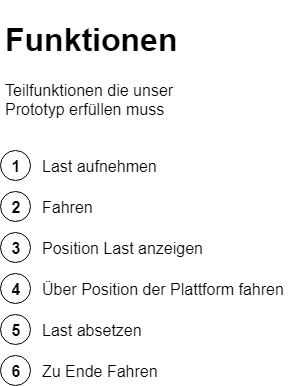
\includegraphics[width=0.5\linewidth,keepaspectratio]{PrototypePlanung}
	\caption{Funktionen Prototyp}
	\label{fig:PrototypePlanung}
\end{figure}

\subsection{Grober Rahmenplan}
\label{ssec:GrobRahmenplan}
An dieser Stelle ist der Projektplan grob umrissen, den Detaillierten finden Sie im Anhang.

\begin{figure}[h!]
	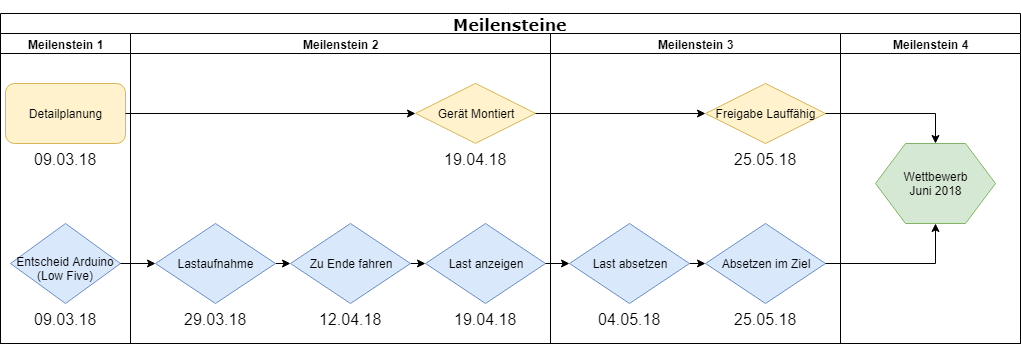
\includegraphics[width=\linewidth,keepaspectratio]{Rahmenplan}
	\caption{Grober Projektplan PREN02}
	\label{fig:GrobProjekt}
\end{figure}

\begin{table}[h!]
\vspace{1em}
\noindent
\begin{tabular}{|p{0.2\textwidth}|p{0.2\textwidth}|p{0.55\textwidth}|}
	\hline
	\textbf{Meileinstein} & \textbf{Termin} & \textbf{Beschreibung} \\
	\hline
	Meilenstein 1 & 09.03.2018 12:00 Uhr & Detailplanung Projekt abgeschlossen, Entscheidung LoFive / Arduino gefallen\\
	\hline
	Meilenstein 2 & 19.04.2018 12:00 Uhr & Steuerungsprototyp v0.3 erreicht, Prototyp  montiert, Vorführung vor Experten\\
	\hline
	Meilenstein 3 & 25.05.2018 12:00 Uhr & Alle Komponenten freigegeben, voller Funktionsumfang erreicht\\
	\hline
	Meilenstein 4 & Juni & Wettbewerb\\
	\hline
	Schlussabgabe PREN2 & TBD & Schlussabgabe Dokumentation zu 100\% fertig \\
	\hline
	\end{tabular}
	\caption{Meilensteine}
	\label{tab:Meilensteine}
\end{table}

\newpage

\section{Budgetplan}
\label{sec:Budgetplan}
Für den Bau der Teilfunktionsmuster in PREN1 dürfen maximal CHF 200.- ausgegeben werden. Die Tabelle \ref{tab:Budgetplan} dient daher vor allem der Kostenverfolgung, damit das Budget nicht überzogen wird.

\vspace{1em}
\noindent
\begin{table}[h!]
	\begin{tabular}{|p{0.3\textwidth}|p{0.15\textwidth}|p{0.225\textwidth}||p{0.225\textwidth}|}
	\hline
	\textbf{Artikel} & \textbf{Anzahl} & \textbf{Preis/Stk. CHF} & \textbf{Total CHF} \\
	\hline
	Rillenkugellager 608-2RS & 1 & 8.36 & 8.36 \\
	\hline
	Rundstab Buche & 3 & 0.9 & 2.7 \\
	\hline
	Buche Rundstäbe glatt & 1 & 0.7 & 0.7 \\
	\hline
	Aluminium Rohmaterial & 1 & 10 & 10 \\
	\hline
	Original Raspberry Pi Kamera Module V2 & 1 & 29.9 & 29.9 \\
	\hline
	Raspberry Pi Model B & 1 & 25.5 & 25.5 \\
	\hline
	Lofive & 1 & 25 & 25 \\
	\hline
	TURNIGY 1800MAH 3S 20C LIPO-PACK & 1 & 25 & 25\\
	\hline
	\textbf{Total} & & & \textbf{127.16} \\
	\hline
	\end{tabular}
	\caption{Budgetplan für das Projekt im PREN01}
	\label{tab:Budgetplan}
\end{table}

\section{Risikomanagement}
\label{ch:RisikoMgmt}
In diesem Kapitel werden mögliche Risiken während des Projektverlaufes aufgelistet. Dabei werden Projektrisiken nummeriert. Ihre Eintrittswahrscheinlichkeit und ihr Schadensausmass wird eingeschätzt. Besteht ein grosses Risiko, werden zusätzlich Massnahmen definiert.

\subsection{Definitionen}
\label{sec:Def}
\vspace{1em}
\noindent
Eintrittswahrscheinlichkeit:

\vspace{1em}
\noindent
\begin{tabular}{|p{0.06\textwidth}|p{0.2\textwidth}|p{0.7\textwidth}|}
	\hline
	\textbf{Stufe} & \textbf{Bezeichnung} & \textbf{Beschreibung} \\
	\hline
	1 & unvorstellbar & Möglich aber eher unwahrscheinlich. Tritt nie oder einmal in 14 Wochen auf \\
	\hline
	2 & unwahrscheinlich & Kann in 14 Wochen 1-5 Mal eintreten\\
	\hline
	3 & vorstellbar & Kann in 14 Wochen 6-8 Mal eintreten \\
	\hline
	4 & wahrscheinlich & Kann in 14 Wochen bis zu 10 Mal eintreten \\
	\hline
	5 & häufig & Kann in 14 Wochen 14 Mal eintreten\\
	\hline
\end{tabular}

\vspace{1em}
\noindent
Schadensausmass:

\vspace{1em}
\noindent
\begin{tabular}{|p{0.06\textwidth}|p{0.2\textwidth}|p{0.7\textwidth}|}
	\hline
	\textbf{Stufe} & \textbf{Bezeichnung} & \textbf{Beschreibung} \\
	\hline
	1 & unwesentlich & Die Aufgabenerfüllung wird höchstens geringfügig beeinträchtigt finanzieller Schaden ist im Rahmen des Projekts nicht beeinflussend. Personenschäden treten nicht auf \\
	\hline
	2 & geringfügig & Wahrnehmbare Gefährdung / Einfluss auf das Projekt. Personenschäden treten nicht auf \\
	\hline
	3 & mittelmässig & Wahrnehmbare Gefährdung / Einfluss auf das Projekt.Finanzieller Schaden strapaziert das Projektbudget
	Personenschäden treten nicht auf \\
	\hline
	4 & kritisch & Starke Gefährdung des Projekts. Finanzieller Schaden übersteigt das Projektbudget massiv. Personenschäden treten geringfügig auf \\
	\hline
	5 & katastrophal & Projektabbruch zur Folge. Finanzieller Schaden kann zum Projektstopp führen. Verletzung der Persönlichkeitsrechte
	\\
	\hline
\end{tabular}


\subsection{Risikokatalog}
\label{sec:Risikokatalog}
Legende:
\begin{itemize}
	\item \textbf{S}chadensausmass bei Eintreffen des Risikos
	\item \textbf{W}ahrscheinlichkeit das Risiko eintrifft
	\item \textbf{K}ategorie: \textbf{T}echnisches oder \textbf{P}rojektbezogenes Risiko
	\item \textbf{A}uswirkung auf das Projekt. Produkt aus S und W
\end{itemize}

\vspace{1em}
\noindent
\begin{tabular}{|p{0.03\textwidth}|p{0.75\textwidth}|p{0.03\textwidth}|p{0.03\textwidth}|p{0.03\textwidth}||p{0.03\textwidth}|}
	\hline
	\textbf{Nr.} & \textbf{Beschreibung / Risiko} & \textbf{K} & \textbf{S} & \textbf{W} & \textbf{A} \\
	\hline
	1 & Datenverlust & P & 5 & 1 & 5\\
	\hline
	2 & Zerstörung elektronischer Komponenten durch ESD & T & 3 & 3 & 9 \\
	\hline
	3 & Störung der Steuerungskomponenten durch Elektromotoren & T & 3 & 2 & 6 \\
	\hline
	4 & Fortbewegungsschwierigkeiten des Gerätes & T & 5 & 2 & 10 \\
	\hline
	5 & Schwankungen des Gerätes & T & 2 & 3 & 6 \\
	\hline
	6 & Probleme beim Transport der Last & T & 4 & 2 & 8 \\
	\hline
	7 & Probleme Fertigung oder Beschaffung Komponenten & P & 2 & 3 & 6 \\
	\hline
	8 & Stop über Zielplatzform schlägt fehl & T & 4 & 2 & 8 \\
	\hline
	9 & Fehlkommunikation im Team & P & 3 & 3 & 9 \\
	\hline
	10 & Teammitglied fällt aus & P & 3 & 2 & 6 \\
	\hline
	11 & Verzug bei Erstellung von Dokumenten & P & 3 & 2 & 6 \\
	\hline
	12 & Gerät startet nicht & T & 5 & 1 & 5 \\
	\hline
\end{tabular}

\subsection{Risikobewertung}
\label{sec:RisikoBewertung}
\begin{figure}[h!]
	\centering
	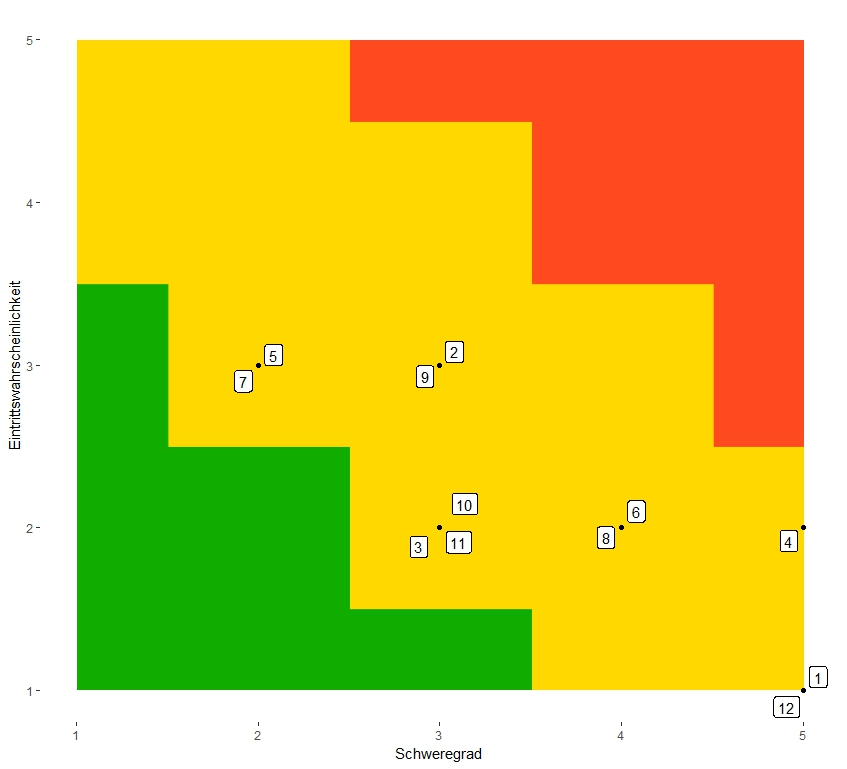
\includegraphics[width=.6\textwidth,keepaspectratio]{Risikomatrix}
	\caption{Die Risiken aus dem Risikokatalog graphisch dargestellt}
	\label{fig:Risikomatrix}
\end{figure}

\newpage
\subsection{Massnahmen}
\label{sec:Massnahmen}
\vspace{1em}
\noindent
\begin{table}[h!]
	\centering
	\begin{tabular}{|p{0.1\textwidth}|p{0.9\textwidth}|}
		\hline
		\textbf{Risiko Nr.} & \textbf{Massnahme} \\
		\hline
		1 & Es wird sowohl für Dokumentation und Programmcode mit GitHub als Versionskontrollsystem gearbeitet. Sonstige Daten befinden sich in der Dropbox. Dropbox wird als sicher eingestuft. \\
		\hline
		2 & Gesamtes Team ist im Umgang mit elektronischen Komponenten geschult. \\
		\hline
		3 & Magnetische Abschirmung des Elektromotors ist vorgesehen. Klare Aufteilung der Printplatte in Digital und Analog. \\
		\hline
		4 & Grösst mögliche Steigung des Seiles wird miteinbezogen. Laufkatze wird gegen rutschen und abstürzen gesichert. Akkuleistung wird genügend gross gewählt. \\
		\hline
		5 & Stabilisierung des Gerätes durch Gewicht oder Dämpfer. \\
		\hline
		6 & Erkennen, greifen und absetzen der Last muss durch Tests in 9 von 10 Mal funktionieren. \\
		\hline
		7 & Aufträge werden frühzeitig in Auftrag gegeben. Vor Auftragserteilung und Bestellung werden diese durch mindestens zwei Personen Überprüft.\\
		\hline
		8 & Zielerkennung wird unter verschiedenen Bedingungen (zum Beispiel Lichteinflüssen) getestet und muss in 9 von 10 Mal funktionieren. Laufkatze soll vor- und rückwärts fahren können. \\
		\hline
		9 & Bei Unklarheiten und Unwohlsein wird von jedem Teammitglied erwartet, dass er sich selbst meldet. Zur Veranschaulichung technischer Aspekte wird mit Skizzen gearbeitet. \\
		\hline
		10 & Aktueller Stand ist zu jedem Zeitpunkt allen klar. Aufgaben-Board ist immer aktuell. Im Falle eines Ausfalls kann so jemand anderes übernehmen. \\
		\hline
		11 & Mit Arbeiten und dazugehöriger Dokumentation wird frühzeitig begonnen. Der Aufwand wird grosszügig mit einberechnet / Puffer. \\
		\hline
		12 & Aufbau der Laufkatze wird geübt und soll nie länger als 1.5min dauern. Das Startsignal soll über zwei Verschiedenen Kanäle gesendet werden können. \\
		\hline
	\end{tabular}
	\caption{Massnahmen welche definiert wurden um die Risiken aus \ref{sec:Risikokatalog} zu minimieren}
	\label{tab:Massnahmen}
\end{table}

\newpage
\subsubsection{Effekt der Massnahmen}
\label{ssec:MassEffekt}
\begin{figure}[h!]
	\centering
	\begin{subfigure}[b]{0.45\textwidth}
		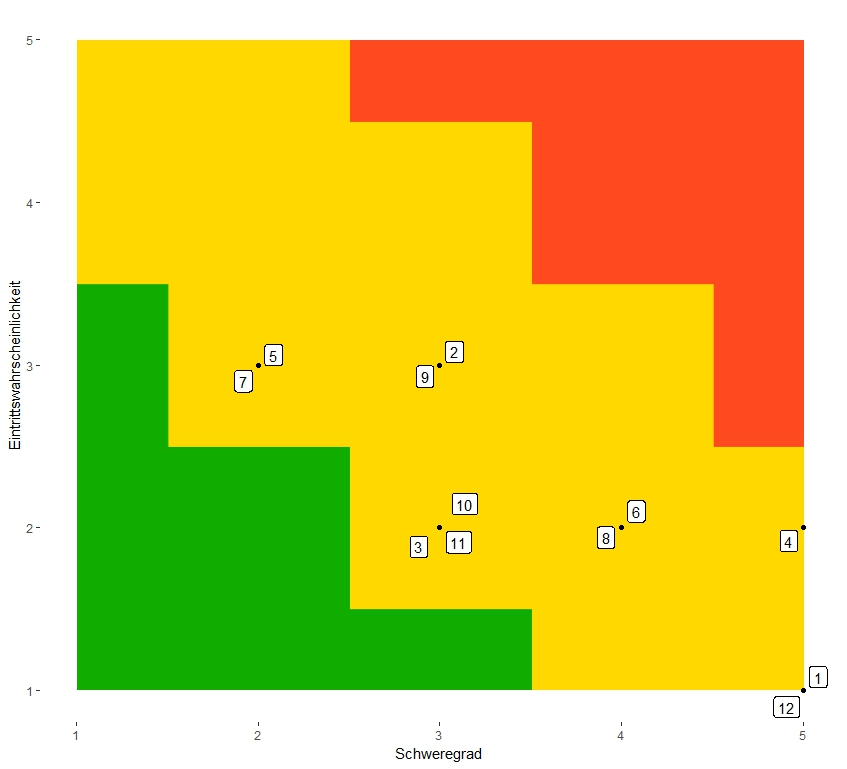
\includegraphics[keepaspectratio,width=\textwidth]{Risikomatrix}
	\end{subfigure}
	\begin{subfigure}[b]{0.45\textwidth}
		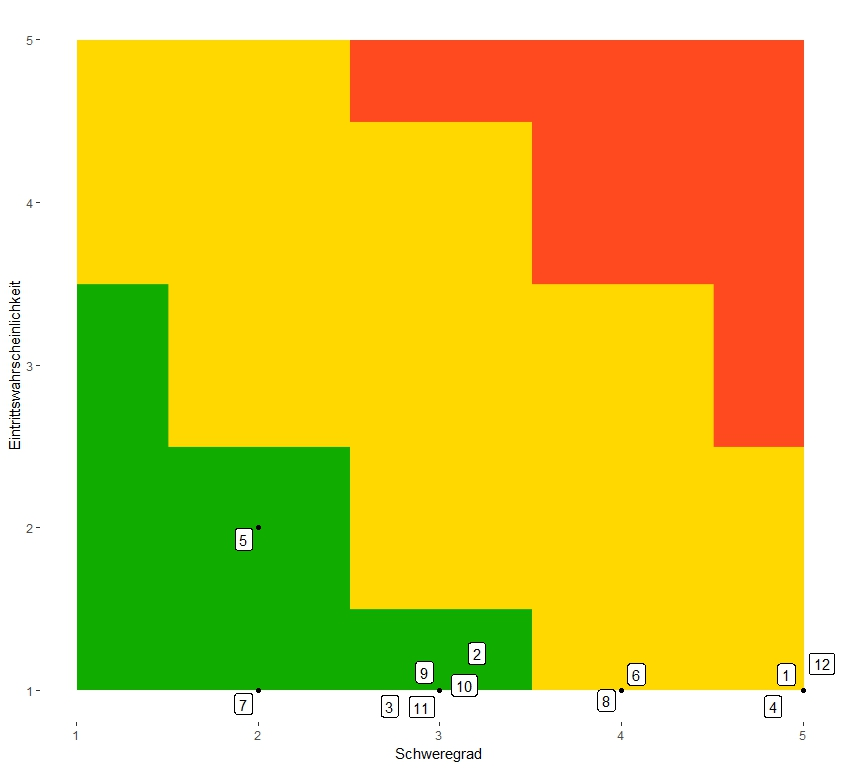
\includegraphics[keepaspectratio,width=\textwidth]{Risikomatrix_nachher}
	\end{subfigure}
	\caption{Gegenüberstellung der Risikomatrizen vor und nach den Massnahmen}
	\label{fig:Gegenueberstellung}
\end{figure}

\begin{figure}[h!]
	\centering
	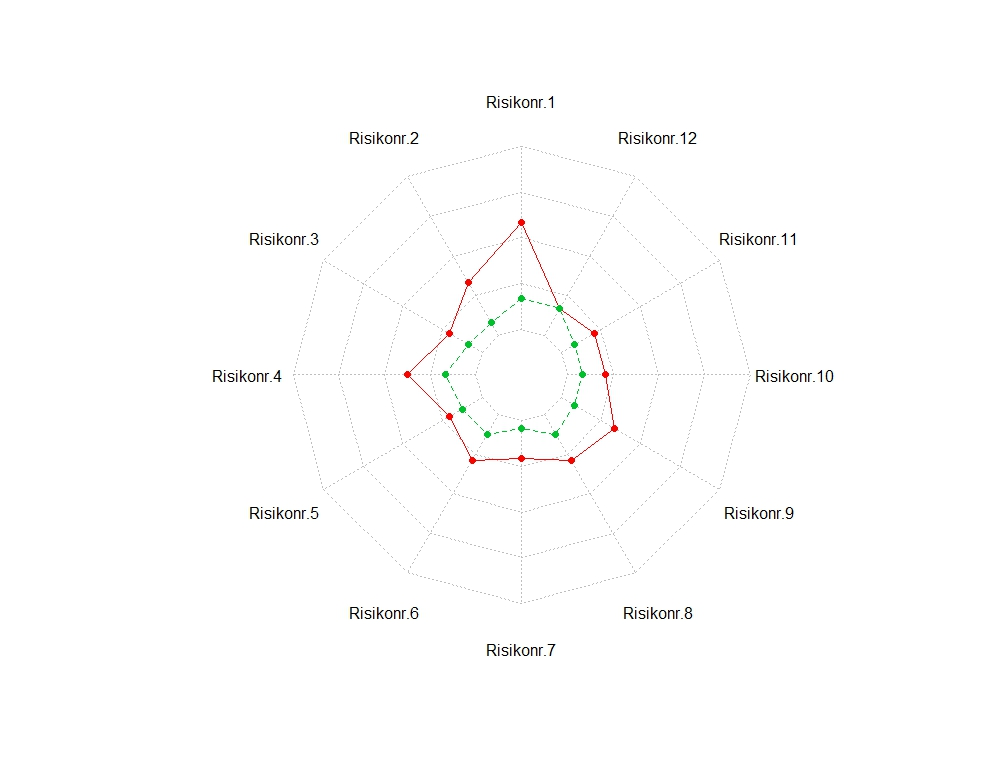
\includegraphics[width=\textwidth,keepaspectratio]{Risikomatrix_Spinne}
	\caption{Die Risiken aus dem Risikokatalog graphisch dargestellt, die rote Linie zeigt die Risiken vor den Massnahmen, während die Grüne die Risiken nach dem Anwenden der Massnahmen darstellt}
	\label{fig:Risikomatrix_Spinne}
\end{figure}


\chapter{Schlussdiskussion}
\label{ch:SchlussDisku}

\listoffigures

\listoftables

\printbibliography

\appendix

\chapter{Aufgabenstellung im Original}
\label{app:ch:AufgabenOriginal}
Die Aufgabenstellung im Original folgt auf den nächsten Seiten.

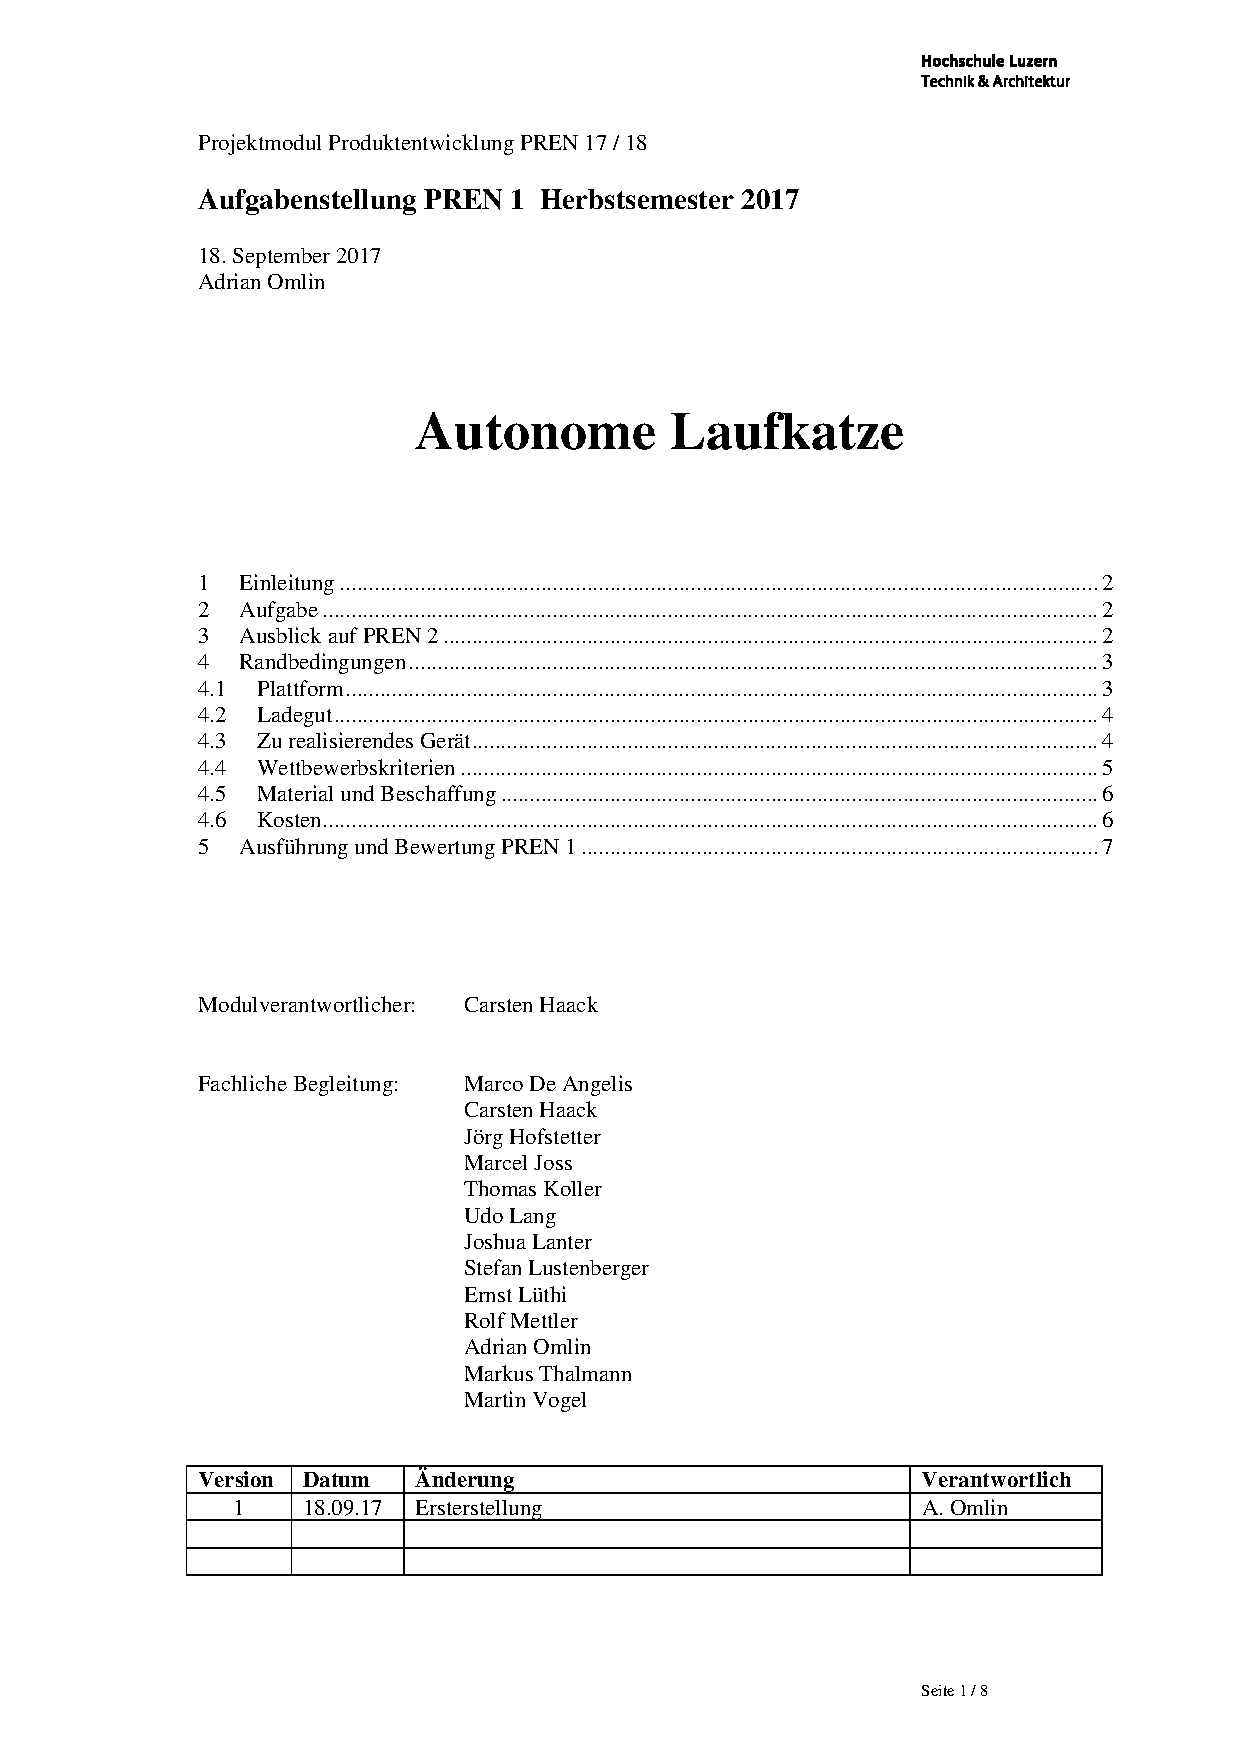
\includepdf[pages=1-8]{AufgabenstellungPREN1H17.pdf}

\chapter{Anforderungen aus PREN 01}
\label{app:ch:Anforderungen}
\section{Projektanforderungen}
\label{app:sec:ProjektAnf}
\begin{tabular}{|p{.05\textwidth}|p{0.07\textwidth}|p{0.3\textwidth}|p{0.55\textwidth}|}
	\hline
	\textbf{Nr.} & \textbf{FMW\footnotemark} & \textbf{Bezeichnung} & \textbf{Beschreibung} \\
	\hline
	1.1 & F & Projektabgabe & Dezember 2017 \\
	\hline
	1.2 & F & Eigenleistung & Systemkomponenten können zugekauft werden \\
	\hline
	1.3 & F & Interdisziplinarität & Disziplinen / Abteilungen arbeiten zusammen \\
	\hline
	1.4 & W & Lieferantenwahl & Für Sammelbestellungen gem. Kapitel 4.5 der Aufgabenstellung. Wird Material vom Team selbst gekauft, können die Kosten zurückgefordert werden \\
	\hline
	1.5 & M & Budget f. PREN & max. 500.- CHF \\
	\hline
	1.6 & M & Teilbudget PREN1 & max. 200.- CHF \\
	\hline
	1.7 & M & 3D-Drucker Laufzeit & max. 25h \\
	\hline
	1.8 & M & Lasergerät Laufzeit & max. 1h \\
	\hline
	1.9 & M & Stunden ET-Werkstattpersonal & max. 10h \\
	\hline
	1.10 & M & Stunden M-Werkstattpersonal & max. 10h \\
	\hline
	1.11 & F & "Gesponsorte"\ Komponenten & Werden mit einem realistischen Preis in die Kostenrechnung einbezogen \\
	\hline
\end{tabular}
\footnotetext{F: Festanforderung M: Mindestanforderung W: Wunschanforderung }

\section{Plattform}
\label{app:sec:Plattform}
\begin{tabular}{|p{.05\textwidth}|p{0.07\textwidth}|p{0.3\textwidth}|p{0.55\textwidth}|}
	\hline
	\textbf{Nr.} & \textbf{FMW\footnotemark} & \textbf{Bezeichnung} & \textbf{Beschreibung} \\
	\hline
	2.1 & F & Gesamtlänge & 350 $\pm$ 2cm \\
	\hline
	2.2 & F & Masten Abstand & Abstand zwischen den Masten 350cm $\pm$ 2cm \\
	\hline
	2.3 & F & Masten Masse & 8cm Front, 6cm Tiefe \\
	\hline
	2.4 & F & Drahtseil & Verzinkter Stahl, Durchmesser 3mm \\
	\hline
	2.5 & F & Seilspannung & Via Umlenkrollen durch ein Gewicht mit einer Masse von 15kg \\
	\hline
	2.6 & F & Winkel des Seiles & 8-20\SI{}{\degree}\\
	\hline
	2.7 & F & Grundplatte & Spanplatte roh oder grau gestrichen.\\
	& & & Mit Farbresten / vorstehenden Schrauben und Nahtstellen ist zu rechnen \\
	\hline
	2.8 & F & Startfeld & 50cm $\pm$ 2cm, Quadratisch \\
	\hline
	2.9 & F & Zielplatte & 31.5cm x 31.5cm \\
	\hline
	2.10 & F & Zielplatte Aussehen & 5 konzentrische Bereiche?\\
	& & & Der innerste, helle Bereich ist quadratisch und hat eine Seitenlänge von 6cm $\pm$ 2mm. \\
	& & & Jeder daran anschliessende konzentrische Bereich hat eine Breite von 2.5cm $\pm$ 2mm. \\
	& & & Die Bereiche sind abwechslungsweise hell und dunkel \\
	\hline
	2.11 & F & Zielplatte Position & Der Absetzbereich verläuft unterhalb des Seiles und ist 2cm breit.\\
	& & & Die Zielplatte kann bis zum Startsignal verschoben werden.\\
	& & & Befindet sich aber immer im Absetzbereich (siehe Abbildung 1 der Aufgabenstellung) \\
	\hline
	2.12 & F & Start- und Zielplatte & Matt \\
	\hline
	2.13 & F & Hindernisse & Auf der gesamten Plattform können Hindernisse stehen.\\
	& & & Im Umkreis von mindestens 10cm um die Startposition des Ladegutes und um die Zielplatte herum sind keine Hindernisse \\
	\hline
	2.14 & M & Hindernisse Höhe & Die Hindernisse haben eine maximale Höhe von 20cm. \\
	\hline
\end{tabular}
\footnotetext{F: Festanforderung M: Mindestanforderung W: Wunschanforderung }

\section{Laufkatze}
\label{app:sec:LaufKatze}
\begin{tabular}{|p{.05\textwidth}|p{0.07\textwidth}|p{0.3\textwidth}|p{0.55\textwidth}|}
	\hline
	\textbf{Nr.} & \textbf{FMW\footnotemark} & \textbf{Bezeichnung} & \textbf{Beschreibung} \\
	\hline
	3.1 & F & Steuerung & Autonom \\
	\hline
	3.2 & M & Inbetriebnahme & Darf max. 2min dauern \\
	\hline
	3.3 & M & Startsignal & Darf per Kopfdruck gesendet werden \\
	\hline
	3.4 & M & Geschwindigkeit & Um die Aufgabe zu bewältigen steht der Laufkatze\\
	& & & ein Zeitfensters von 4min zur Verfügung. \\
	\hline
	3.5 & M & Aussendimensionen & Die Laufkatze darf in ihrer Projektion das Startfeld nicht überschreiten. 50cm $\pm$ 2cm x 50cm $\pm$ 2cm \\
	\hline
	3.6 & F & Bauart & Sämtliche Sensorik muss auf dem Gerät selbst montiert sein. \\
	\hline
	3.7 & F & Fahrweise & Das Gerät darf nur das Drahtseil und den zweiten Masten berühren.\\
	& & & Die gesamte Plattform, insbesondere Drahtseil, die Last und die Zielplatte dürfen nicht beschädigt oder sonst irgendwie verändert werden.\\
	& & & Es ist beispielsweise nicht erlaubt, Navigationshilfen anzubringen. \\
	\hline
	3.8 & F & Ladegut & Das Gerät muss ein Ladegut transportieren können. \\
	\hline
	3.9 & F & Zielerkennung & Das Erkennen der Zielplatte muss selbstständig erfolgen\\
	\hline
\end{tabular}
\footnotetext{F: Festanforderung M: Mindestanforderung W: Wunschanforderung }

\section{Ladegut}
\label{app:sec:AnfLadegut}
\begin{tabular}{|p{.05\textwidth}|p{0.07\textwidth}|p{0.3\textwidth}|p{0.55\textwidth}|}
	\hline
	\textbf{Nr.} & \textbf{FMW\footnotemark} & \textbf{Bezeichnung} & \textbf{Beschreibung} \\
	\hline
	4.1 & F & Material & Holz \\
	\hline
	4.2 & F &  Dimensionen & Seitenlänge 5cm $\pm$ 0.5cm \\
	\hline
	4.3 & M & Gewicht & 50-90g, siehe Sektion \ref{app:sec:RechKlotzMasse} \\
	\hline
	4.4 & F & Aufnahme & Metallischer, magnetischer Haken oben in der Mitte des Würfels.\\
	& & & Innendurchmesser des Hakens ist 1.3cm $\pm$ 0.1mm\\
	\hline
	4.5 & F & Hindernisse & Das Ladegut darf Hindernisse nicht berühren. \\
	\hline
	4.6 & F & Position & Die Position des Ladegutes muss in Echtzeit angezeigt werden, dass der Schiedsrichter jederzeit die angezeigten Werte gut erkennen kann.\\
	\hline
	4.7 & F & Positionsbestimmung & Die Mitte des Bodens des Ladegutes wird verwendet.\\
	& & & Die Position muss in x- und z-Richtung bestimmt werden (siehe Skizze Anforderungen).\\
	& & & Der Nullpunkt des zu verwendenden Koordinatensystems ist in Abbildung 1 der Aufgabenstellung definiert. \\
	\hline
	4.8 & F & Absetzen & Das Ladegut muss innerhalb des Zielbereiches automatisch abgesetzt werden. \\
	\hline
	4.9 & F & Zielbereich & Der Zielbereich muss automatisch erkennt werden\\
	\hline
\end{tabular}
\footnotetext{F: Festanforderung M: Mindestanforderung W: Wunschanforderung }

\section{Umfeld}
\label{app:sec:Umfeld}
\begin{tabular}{|p{.05\textwidth}|p{0.07\textwidth}|p{0.3\textwidth}|p{0.55\textwidth}|}
	\hline
	\textbf{Nr.} & \textbf{FMW\footnotemark} & \textbf{Bezeichnung} & \textbf{Beschreibung} \\
	\hline
	5.1 & M & Licht & Scheinwerfer welche auf die Wettbewerbsplattformen gerichtet sind, werden dazu führen, dass wir mit einer hohen Helligkeit arbeiten müssen \\
	\hline
	5.2 & M & Temperaturen & Bei Lagerung und Betrieb Zimmertemperatur 15-\SI{20}{\degreeCelsius}\\
	\hline
	5.3 & M & Kein Spritzwasser & Für Innenanwendung\\
	\hline
	5.4 & M & Keine Hochspannung & Normale Netzspannung\\
	\hline
	5.5 & M & Raumhöhe & Als Wettbewerbsraum wird eine Normale Raumhöhe (2.5-3m) angenommen.\\
	\hline
\end{tabular}
\footnotetext{F: Festanforderung M: Mindestanforderung W: Wunschanforderung }

\chapter{Versuche}
\label{app:ch:Versuche}

Anhand von Aufgabenstellung, Anforderungen und Risikomanagement ist klar, welche Schnittstellen und/oder Teilkomponenten besonders wichtig sind. Zu den wichtigsten Schnittstellen und/oder Teilkomponenten wurden Versuche durchgeführt, welche entweder eine positive Eigenschaft bestätigen, oder eine negative Eigenschaft hervorheben. Die detaillierten Testprotokolle zu den jeweiligen Versuchen sind im Anhang \ref{app:ch:Versuche}.

\subsection{Aufhängung und Antrieb}
In einem ersten Versuch (Anhang \ref{app:ch:Versuche} Testprotokoll Laufkatze + Antrieb\_V1) wurde festgestellt, dass sich die Konstruktion nicht genügend Symmetrisch verhält. Dadurch hängt die Last nicht direkt unter dem Antrieb, sondern kann sich bis zu 1cm nach vorne und nach hinten versetzen. Ob der Versatz nach vorne oder nach hinten ist, hängt von den einwirkenden Beschleunigungen (positiv oder negativ) ab. So können Probleme bei der Positions- und Zielerkennung entstehen. Es muss ein neuer Prototyp ohne Selbstspannmechanismus konstruiert, hergestellt und getestet werden.

Im zweiten Versuch (Testprotokoll Laufkatze + Antrieb\_V2) wurde dann der Prototyp 2 des Antriebes und der Aufhängung getestet. Das Problem des Versatzes in x-Richtung bzw. Pendeln um die y-Achse war damit behoben. Auch die Einstellung der Spannkraft funktioniert gut, sodass kein Selbstspannmechanismus nötig ist. Die nötige Vorspannkraft, mit welcher die Reibungskraft erhöht werden kann, muss während dem Modul PREN2 noch ermittelt werden.

\subsection{Schrittmotoren}
Zum Fortbewegen sowie zum Anheben der Last werden Schrittmotoren eingesetzt. Damit darauf aufbauend Tests fürs Fahren sowie das Lastanheben möglich sind werden die Motoren mit einem Laboraufbau getestet. Angetrieben werden die Schrittmotoren von einem Microchip, welcher spezifisch für dessen Ansteuerung ausgelegt ist.

Mit dem ersten Aufbau kommt der Motor nicht in Bewegung. Darauf folgend wird die Treiberkomponente mit dem Oszilloskop und der Schrittmotor mit einem anderen Ansteuerungs-Modul getestet. So konnte erkannt werden, dass der Motor einwandfrei funktioniert, die Treiberkomponente jedoch einen Defekt hat. Daher muss für einen weiteren Testlauf eine neue Treiberkomponente angeschafft werden.

\subsection{Durchhang}
\label{ssec:VersDurch}
Durch Anhängen eines Gewichtes in regelmässigen Abständen und über die ganze Strecke verteilt, wurde der jeweilige Durchhang gemessen und danach in einer Excel-Tabelle eingetragen. Durch Erstellen eines Diagramms konnte für die Kurve eine Trendlinie erstellt werden. Aus dieser konnte eine Funktion des Durchhanges in Abhängigkeit der Strecke abgeleitet werden. Mit dieser Funktion (siehe Abbildung \ref{fig:Durchhang_v1}) kann später auch die Position ermittelt werden.
\begin{figure}[h!]
	\centering
	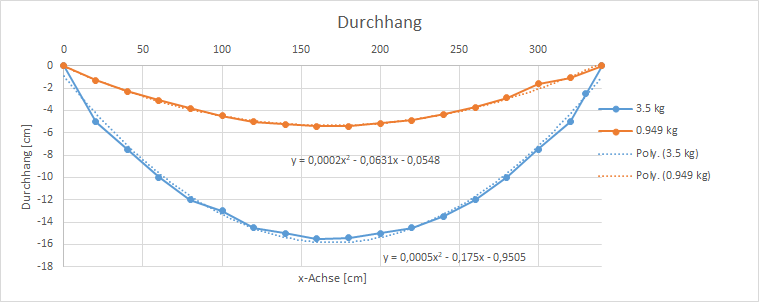
\includegraphics[width=\textwidth,keepaspectratio]{Durchhang_v1}
	\caption{Diagramm zum Durchhang}
	\label{fig:Durchhang_v1}
\end{figure}

Interessant ist, dass die tatsächlichen Werte des Durchhanges schlecht mit den errechneten Werten in Tabelle \ref{tbl:DurchhangRechnung} übereinstimmten. Dies führt daher, dass die Umlenkrollen der Plattform eine grosse Reibung aufweisen und daher die Rechnung mit konstanter Seilspannung eigentlich nicht ganz richtig ist. Die Rollen werden, jedoch von der Modulleitung noch durch reibungsärmere ersetzt. Danach muss die Durchhangsmessung erneut durchgeführt werden. Das detaillierte Protokoll ist im im Anhang \ref{app:ch:Versuche} "Testprotokoll Versuch Durchhang".

\subsection{Last greifen \& absetzen}
\label{ssec:VersLastg}

Für einen Mechanismus um die Last zu Greifen, fiel die erste Wahl ursprünglich auf eine Konstruktion mit Elektromagnet. Diesen Elektromagneten wollten wir selbst bauen. Das Testprotokoll \textquotedblleft Elektromagnet V1\textquotedblright\ (Anhang \ref{app:ch:Versuche}) zeigt, dass die Last zwar angehoben werden konnte, der Elektromagnet jedoch sehr heiss wurde. Dies aufgrund der hohen Leistung von 4W welche durch die Spule fliesst.

Nach dem Versuch \textquotedblleft Elektromagnet V2\textquotedblright\ (Anhang \ref{app:ch:Versuche})wurde klar, dass durch die vorgenommenen Änderungen der Elektromagnet nur noch am Rand eine magnetische Wirkung besitzt.

Um eine Alternative ohne Elektromagnet zu testen, wurde ein Prototyp gebaut um die Teilfunktion \textquotedblleft Last greifen\textquotedblright\ durch einen Haken umzusetzen.

Der Versuch \textquotedblleft Last Greifen mit Haken\textquotedblright\ (Anhang \ref{app:ch:Versuche}) hat gezeigt, dass die gelenkig gelagerte Hakenkonstruktion sich gut eignet um die Last mittig anzuheben. Ausserdem hat der Versuch gezeigt, dass durch Berührung der Last, der Haken nach hinten gekippt wird und die Last dadurch nicht verschoben wird. Das Absetzen der Last wir im Versuchsprotokoll \textquotedblleft Last absetzen mit Haken\textquotedblright\ (Anhang \ref{app:ch:Versuche}) beschrieben. Änderungen an der Geometrie des Greifers sind momentan nicht vorgesehen.

\subsection{Entwicklungsumgebung Informatik}
\label{ssec:VersEntI}
Ziel war es sicherzustellen, dass eine Entwicklungsumgebung zur Bilderkennung mit den bisher vorgesehenen Komponenten möglich ist. Der Versuch war erfolgreich und lieferte alle erwarteten Resultate. Das detaillierte Protokoll findet man im Anhang \ref{app:ch:Versuche} \textquotedblleft Testprotokoll – Entwicklungsumgebung Informatik\textquotedblright.
Zusätzlich wurde eine Installationsanleitung (\textquotedblleft Raspy Install\textquotedblright Anhang \ref{app:ch:Versuche}) erstellt.

\subsection{Test Zielplatten Erkennung Informatik}
\label{ssec:ZielplattenErkennung}
Ziel war es, die Zielplatte mittels der Programmbibliothek OpenCV zu erkennen (Testprotokoll - Erkennung Zielplatte,Anhang \ref{app:ch:Versuche}).
Die Zielplatte konnte grundsätzlich erkannt werden. Es stellt sich jedoch heraus, dass sobald die Lichtverhältnisse stark ändern, eine Erkennung nicht mehr möglich ist. Zudem wird die Zielplatte nicht erkannt, sobald eine der konzentrischen Bereiche / Linien durchtrennt wird. Sobald ein Hindernis, die zu hebende Last oder Teile unseres Fahrzeuges im Weg sind, funktioniert dieser erste Prototyp der Zielplattenerkennung nicht.

Um zu wissen ob und und mit welchen Bildstörungen zu rechnen sein wird, wurde ein weitere Versuch \textquotedblleft Kameraausrichtung\textquotedblright\ (Anhang \ref{app:ch:Versuche}) durchgeführt.

\subsection{Kameraausrichtung}
\label{ssec:VersKamera}
Ziel war es die Kameraausrichtung am Fahrzeug festzulegen und zu wissen ob und mit welchen Bildstörungen zu rechnen sein wird.
Die Kamera wird ausserhalb des Geräts angebracht um eine Überbelichtung des Sensors zu verhindern (bzw. gleichmässige Lichtverhältnisse im ganzen Bild zu erhalten).
Dieser Versuch bestätigte das Risiko, dass die Zielplatte nicht erkannt wird, sobald Störfaktoren wie Teleskoparm und/oder die Last selbst im Bild sind.  Mit der optimalen Ausrichtung der Kamera, können solche Störfaktoren vermindert, jedoch nicht komplett ausgeschlossen werden. Das detaillierte Protokoll ist im Anhang \ref{app:ch:Versuche}  \textquotedblleft Testprotokoll Kameraausrichtung\textquotedblright.

\subsection{Kommunikation ET - IT Board}
\label{ssec:VersKomm}
Ziel war es, die Kommunikation via UART zwischen Elektronik-Board und Informatik-Board sicherzustellen. Sie wird hauptsächlich dazu gebraucht, damit das Informatik-Board die Erkennung der Zielplatte an das steuernde Elektronik-Board weitergeben kann. Der Versuch wurde nicht fertiggestellt und ist Gegenstand von PREN2.

\chapter{Berechnungen}
\label{app:ch:Berechnung}
\section{Teleskop}
\label{app:sec:Teleskjope}
\subsection{Teleskop Variante 1}
\label{app:ssec:TeleskopjeVar1}
\begin{figure}[h]
	\centering
	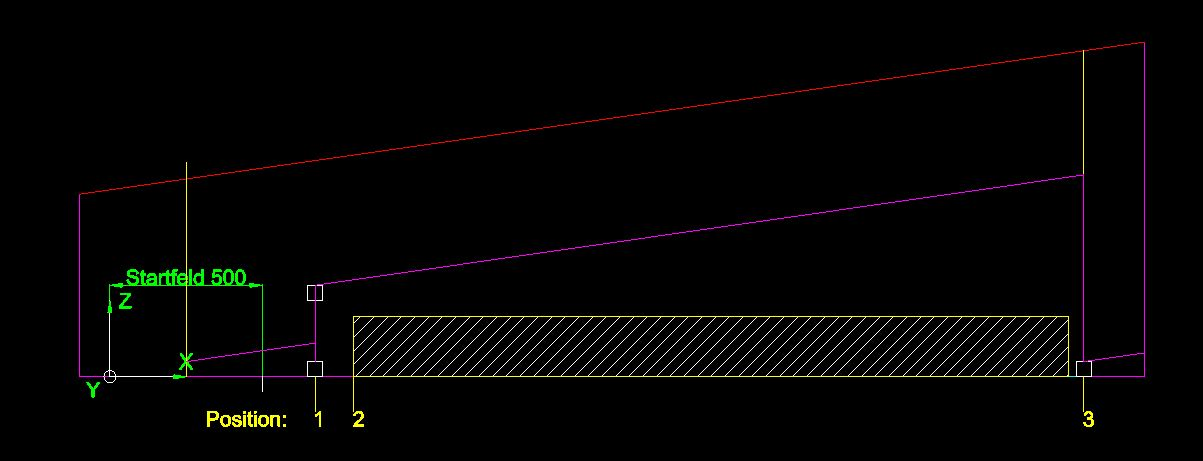
\includegraphics[keepaspectratio,height=4cm]{Teleskoparm1.JPG}
	\caption{Skizze Verfahrweg}
	\label{fig:Skizze Verfahrweg}
\end{figure}

Durch den Weg der die Last zurücklegen muss (violetter Pfad Abbildung \ref{fig:Skizze Verfahrweg}) ergeben sich zwei Extrempositionen.
(Seildurchhang wurde vernachlässigt)


\begin{itemize}[noitemsep]
	\item Position 2: Teleskoparm gestaucht
	\item Position 3: Teleskoparm maximal ausgefahren
\end{itemize}


\begin{figure}[h]
	\centering
	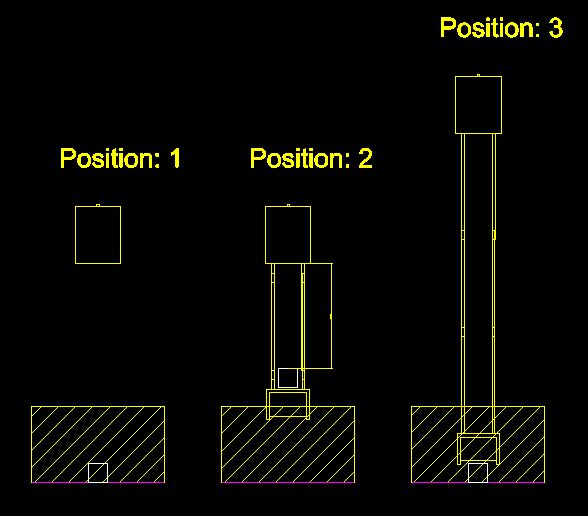
\includegraphics[keepaspectratio,height=4cm]{Teleskoparm2.JPG}
	\caption{Skizze Teleskop}
	\label{fig:Teleskoparm}
\end{figure}

Dabei wurde festgestellt, dass bei Position 2 wesentlich weniger Platz zwischen last und gerät vorhanden ist als bisher angenommen (Abbildung \ref{fig:Teleskoparm}). Bisher wurde mit einem Teleskop gerechnet, welcher aus 3-4 Segmenten besteht. Jedoch lässt sich dies nicht realisieren, da zu wenig Platz vorhanden ist. Für eine solche Lösung wäre ein Teleskop mit mehr als 8 Segmenten nötig. Dies wurde aufgrund des großen Aufwandes verworfen.

\subsection{Teleskop Variante 2}
\label{app:ssec:Teleskopje2}
Deshalb wurde eine Alternativlösung (Abbildung \ref{fig:Linearaufzug}) erarbeitet, bei der die Führungsstäbe nicht wie beim Teleskop eingefahren wird sondern seitwärts neben dem Antriebsmodul vorbei geschoben wird. Dies vereinfacht die bisherige Konstruktion zwar, jedoch muss der Abstand zwischen den Führungen genügend gross sein, dass die Antriebseinheit dazwischen platz hat.

\begin{figure}[h]
	\centering
	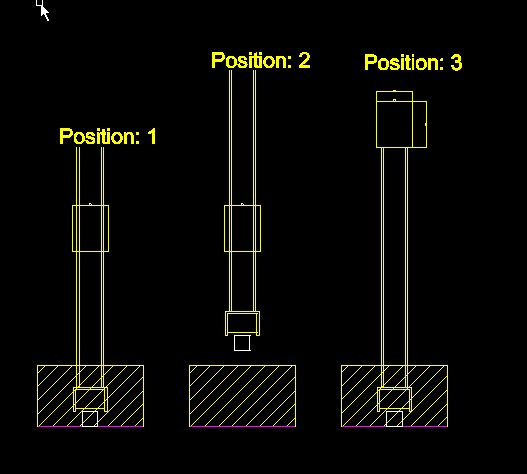
\includegraphics[keepaspectratio,height=4cm]{Teleskoparm3.JPG}
	\caption{Skizze Teleskoparm überarbeitet}
	\label{fig:Linearaufzug}
\end{figure}


\section{Durchhang}
\label{app:sec:Durchhang}
Der Durchhang des Seils ist abhängig vom Gewicht der Laufkatze. Dabei ist es wichtig den Durchhang für das sichere Überfahren der Hindernisse zu kennen. Zudem besteht die Möglichkeit, die Positionsanzeige in vertikaler Richtung als Funktion der zurückgelegten Strecke abzubilden, womit ein zusätzliches Messsystem weggelassen werden kann.

\subsection{Rechnung Durchhang}
\label{ssec:RechDurch}
Die Grundsteigung des Tragseils beträgt 8,2 Grad. Mithilfe von Trigonometrie und der Spannung des Seils konnte der Durchhang in der Mitte des Tragseils näherungsweise ausgerechnet werden.

\vspace{1em}
\noindent
\begin{table}[h!]
	\begin{tabular}{|p{0.15\textwidth}|p{0.2\textwidth}|p{0.55\textwidth}|}
		\hline
		\textbf{Gewicht [kg]} & \textbf{Steigungswinkel [\SI{}{\degree}](ohne Grundsteigung)} &\textbf{Durchhang [cm]}\\
		\hline
		0.5&0,95&2.29\\
		\hline
		1&1,91&5,84\\
		\hline
		1.5&2,87&8,76\\
		\hline
		2&3,82&11,69\\
		\hline
		2.5&4,78&14,63\\
		\hline
		3&5,74&17,59\\
		\hline
		3.5&6,70&20,56\\
		\hline
		4&7,66&23,54\\
		\hline
		4.5&8,63&26,55\\
		\hline
		5&9,59&29,58\\
		\hline
	\end{tabular}
	\caption{Rechnung Durchhang}
	\label{tbl:DurchhangRechnung}
\end{table}


\subsection{Grobversuch Durchhang}
\label{app:ssec:GrobeversDurch}
Es wurde ein einfacher Versuch über den Durchhang des Tragseiles gemacht. Die Dimensionen und Proportionen sind nicht massstäblich, nur Beispielhaft. Dabei wurde ein Seil zwischen zwei Stühlen durch ein Gewicht gespannt. Ein angebrachtes Gewicht wurde dannach an verschiedenen Positionen angehängt und der Durchhang wurde gemessen. Dabei kam raus, dass der maximale Durchhang in der Mitte des Tragseils ist. Der Durchhang im oberen fünftel des Tragseils betrug dabei ungefähr 2/3 des maximalen Durchhangs.
Für eine genaue Funktion des Durchhangs könnten am Musteraufbau Gewichte an verschiedenen Positionen angehängt und der Durchhang von Hand messen. Durch Eingabe in Excel kann somit die Funktion für verschiedene Gewichte ermittelt werden.

\chapter{Meilensteinberichte}
\label{app:ch:MeilensteinBerichte}

\end{document}